%%%%%%%%%%%%%%%%%%%%%%%%%%%%%%%%%%%%%%%%%%%%%%%%%%%%%%%%%%%%%%%%
%%%%%%%%%%%%%%%%%%%%%%%%%%%%%%%%%%%%%%%%%%%%%%%%%%%%%%%%%%%%%%%%
%%%%
%%%% This text file is part of the source of slides for
%%%% `Introduction to High-Performance Scientific Computing'
%%%% by Victor Eijkhout, copyright 2012-2021
%%%%
%%%%%%%%%%%%%%%%%%%%%%%%%%%%%%%%%%%%%%%%%%%%%%%%%%%%%%%%%%%%%%%%
%%%%%%%%%%%%%%%%%%%%%%%%%%%%%%%%%%%%%%%%%%%%%%%%%%%%%%%%%%%%%%%%

\begin{frame}{Summing forces}
  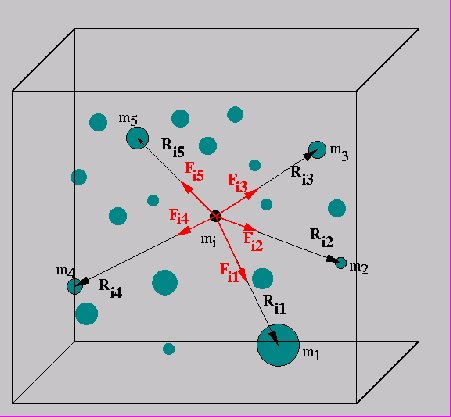
\includegraphics[scale=.4]{nbody_pic}
\end{frame}

\begin{frame}{Particle interactions}
  \begin{tabbing}
    for \=each particle $i$\\
    \>for \= each particle $j$\\
    \>\> let $\bar r_{ij}$ be the vector between $i$ and $j$;\\
    \>\> then the force on $i$ because of $j$ is\\
    \>\> $\quad f_{ij} = -\bar r_{ij}\frac{m_im_j}{|r_{ij}|}$\\
    \>\> (where $m_i,m_j$ are the masses or charges) and\\
    \>\> $f_{ji}=-f_{ij}$.\\
    \>Sum forces and move particle over $\Delta t$\\
  \end{tabbing}
\end{frame}

\begin{frame}{Complexity reduction}
  \begin{itemize}
  \item Naive all-pairs algorithm: $O(N^2)$
  \item Clever algorithms: $O(N\log N)$, sometimes even~$O(N)$
  \item Octtree algorithm: Barnes-Hut
  \end{itemize}  
\end{frame}

\begin{frame}{Octtree}
    \hbox{%
  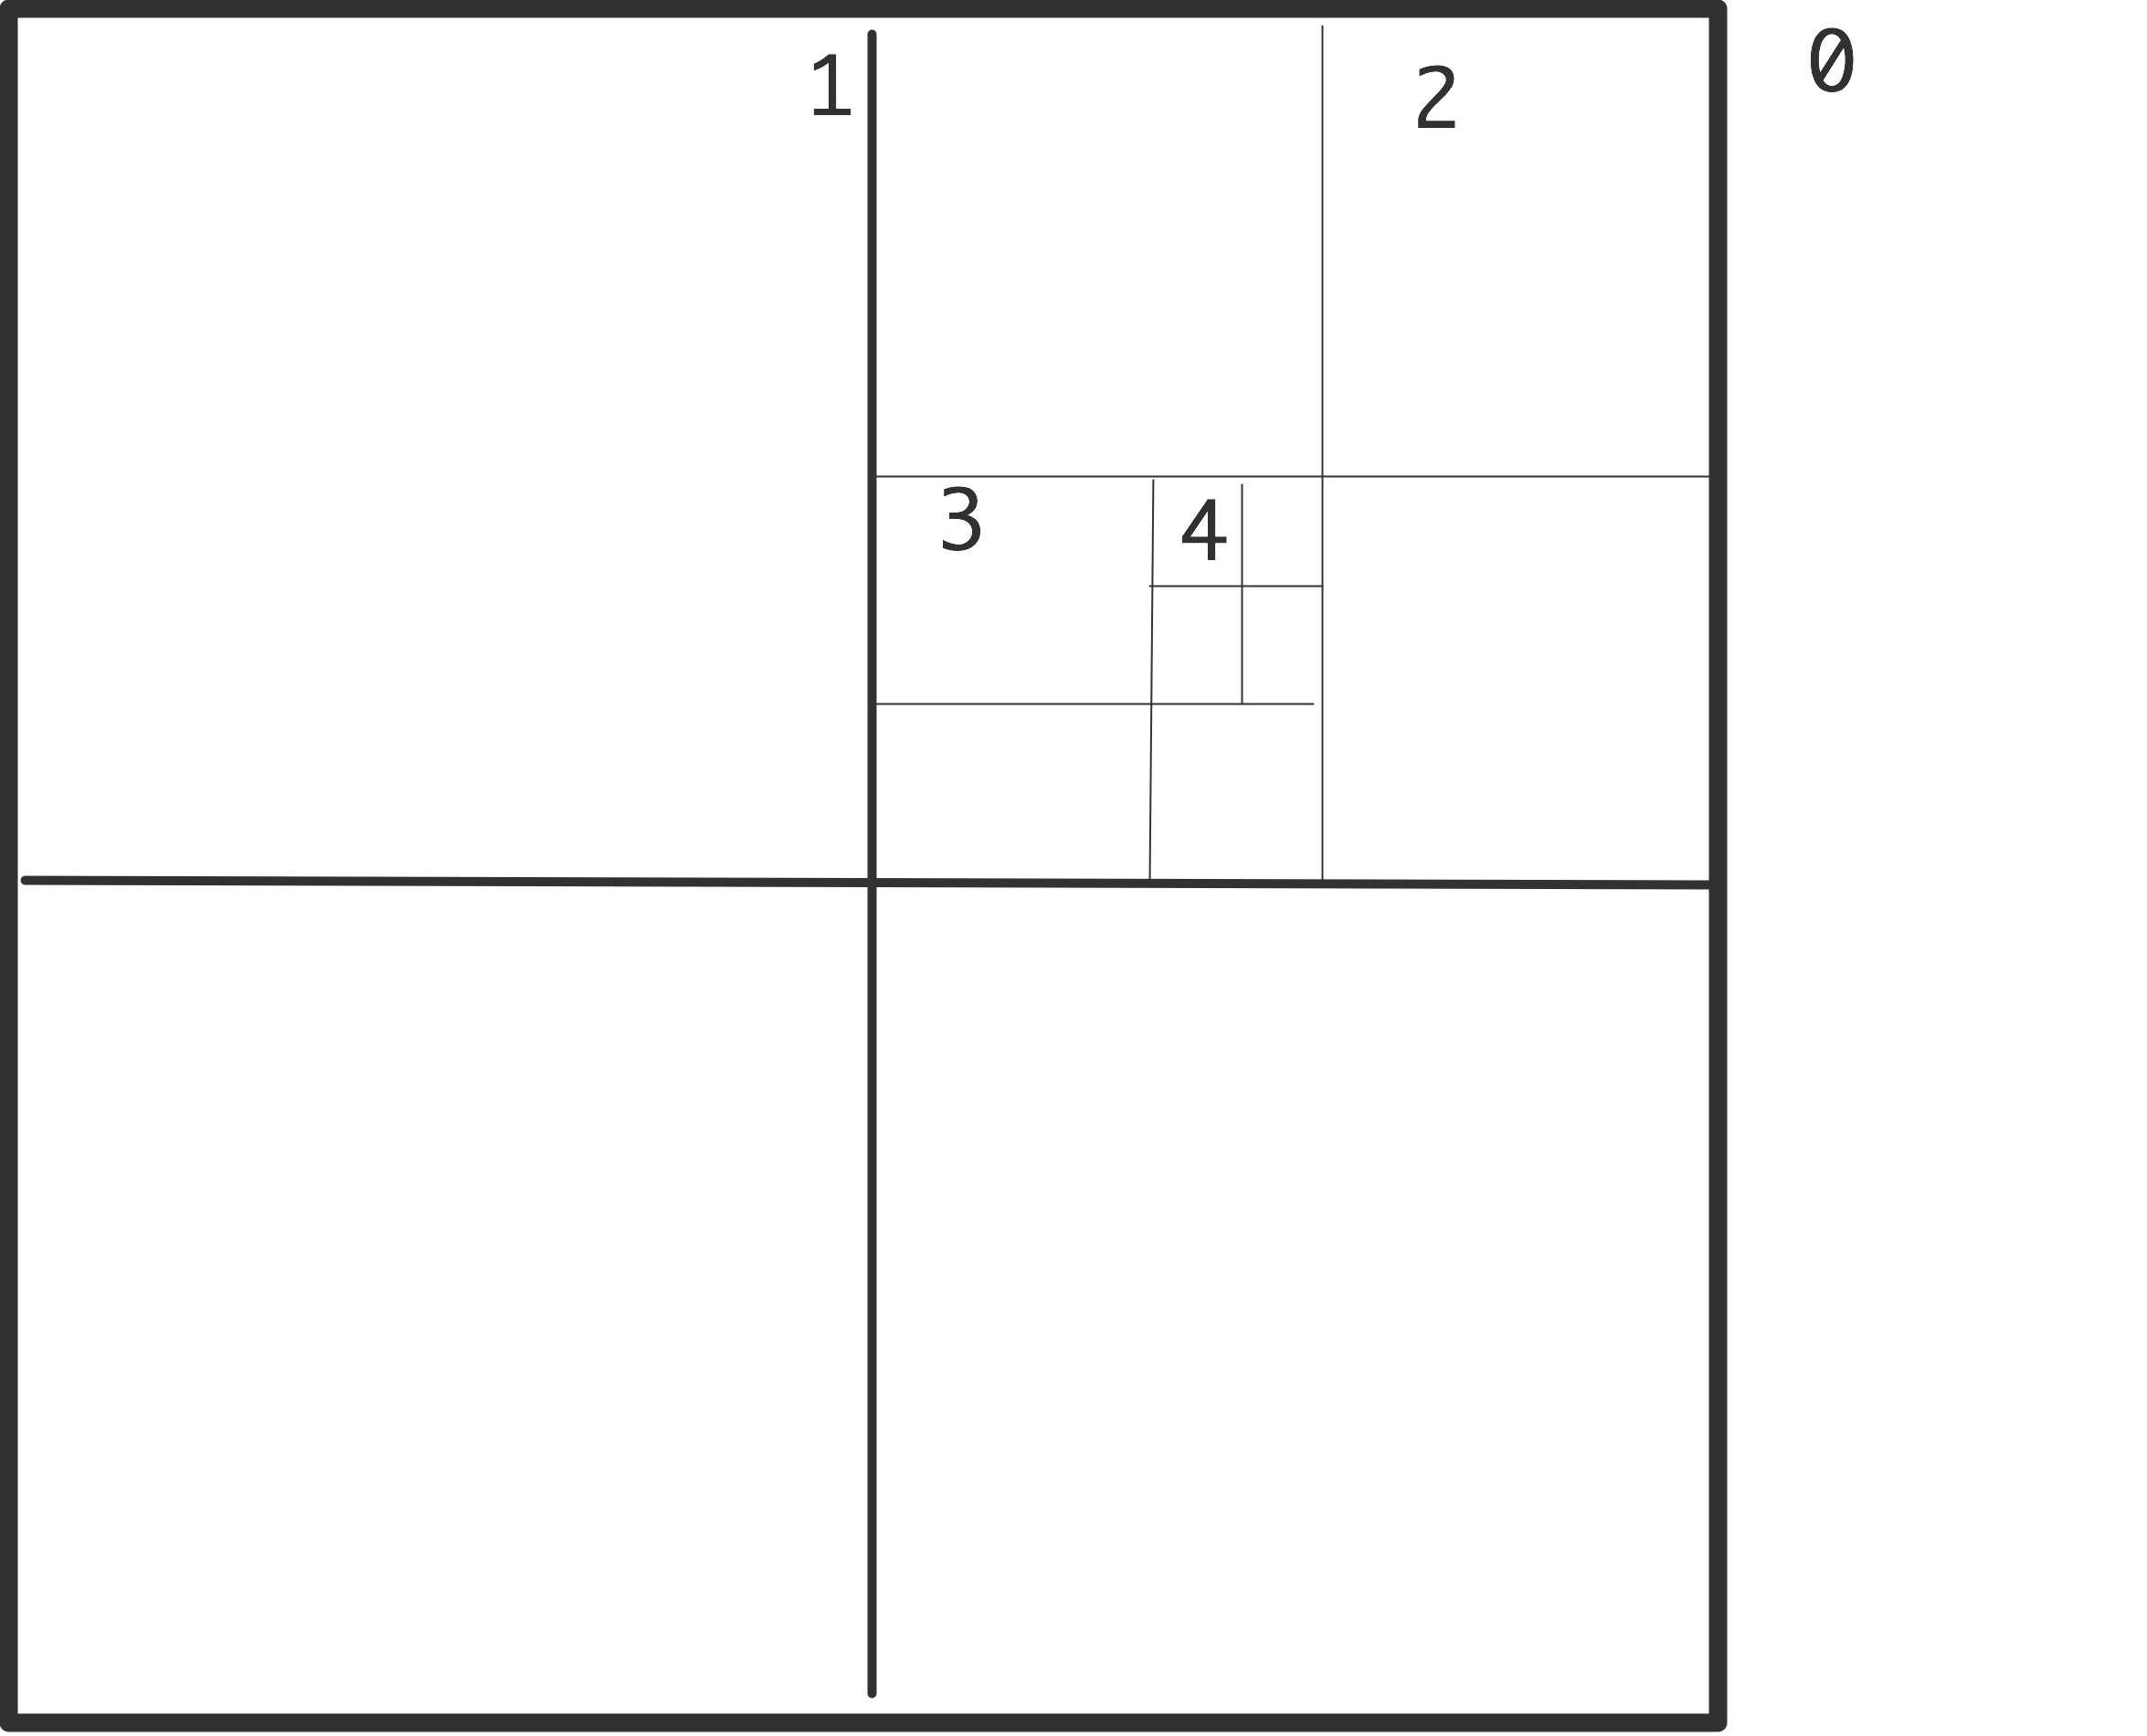
\includegraphics[scale=.05]{bh-quadrants}
  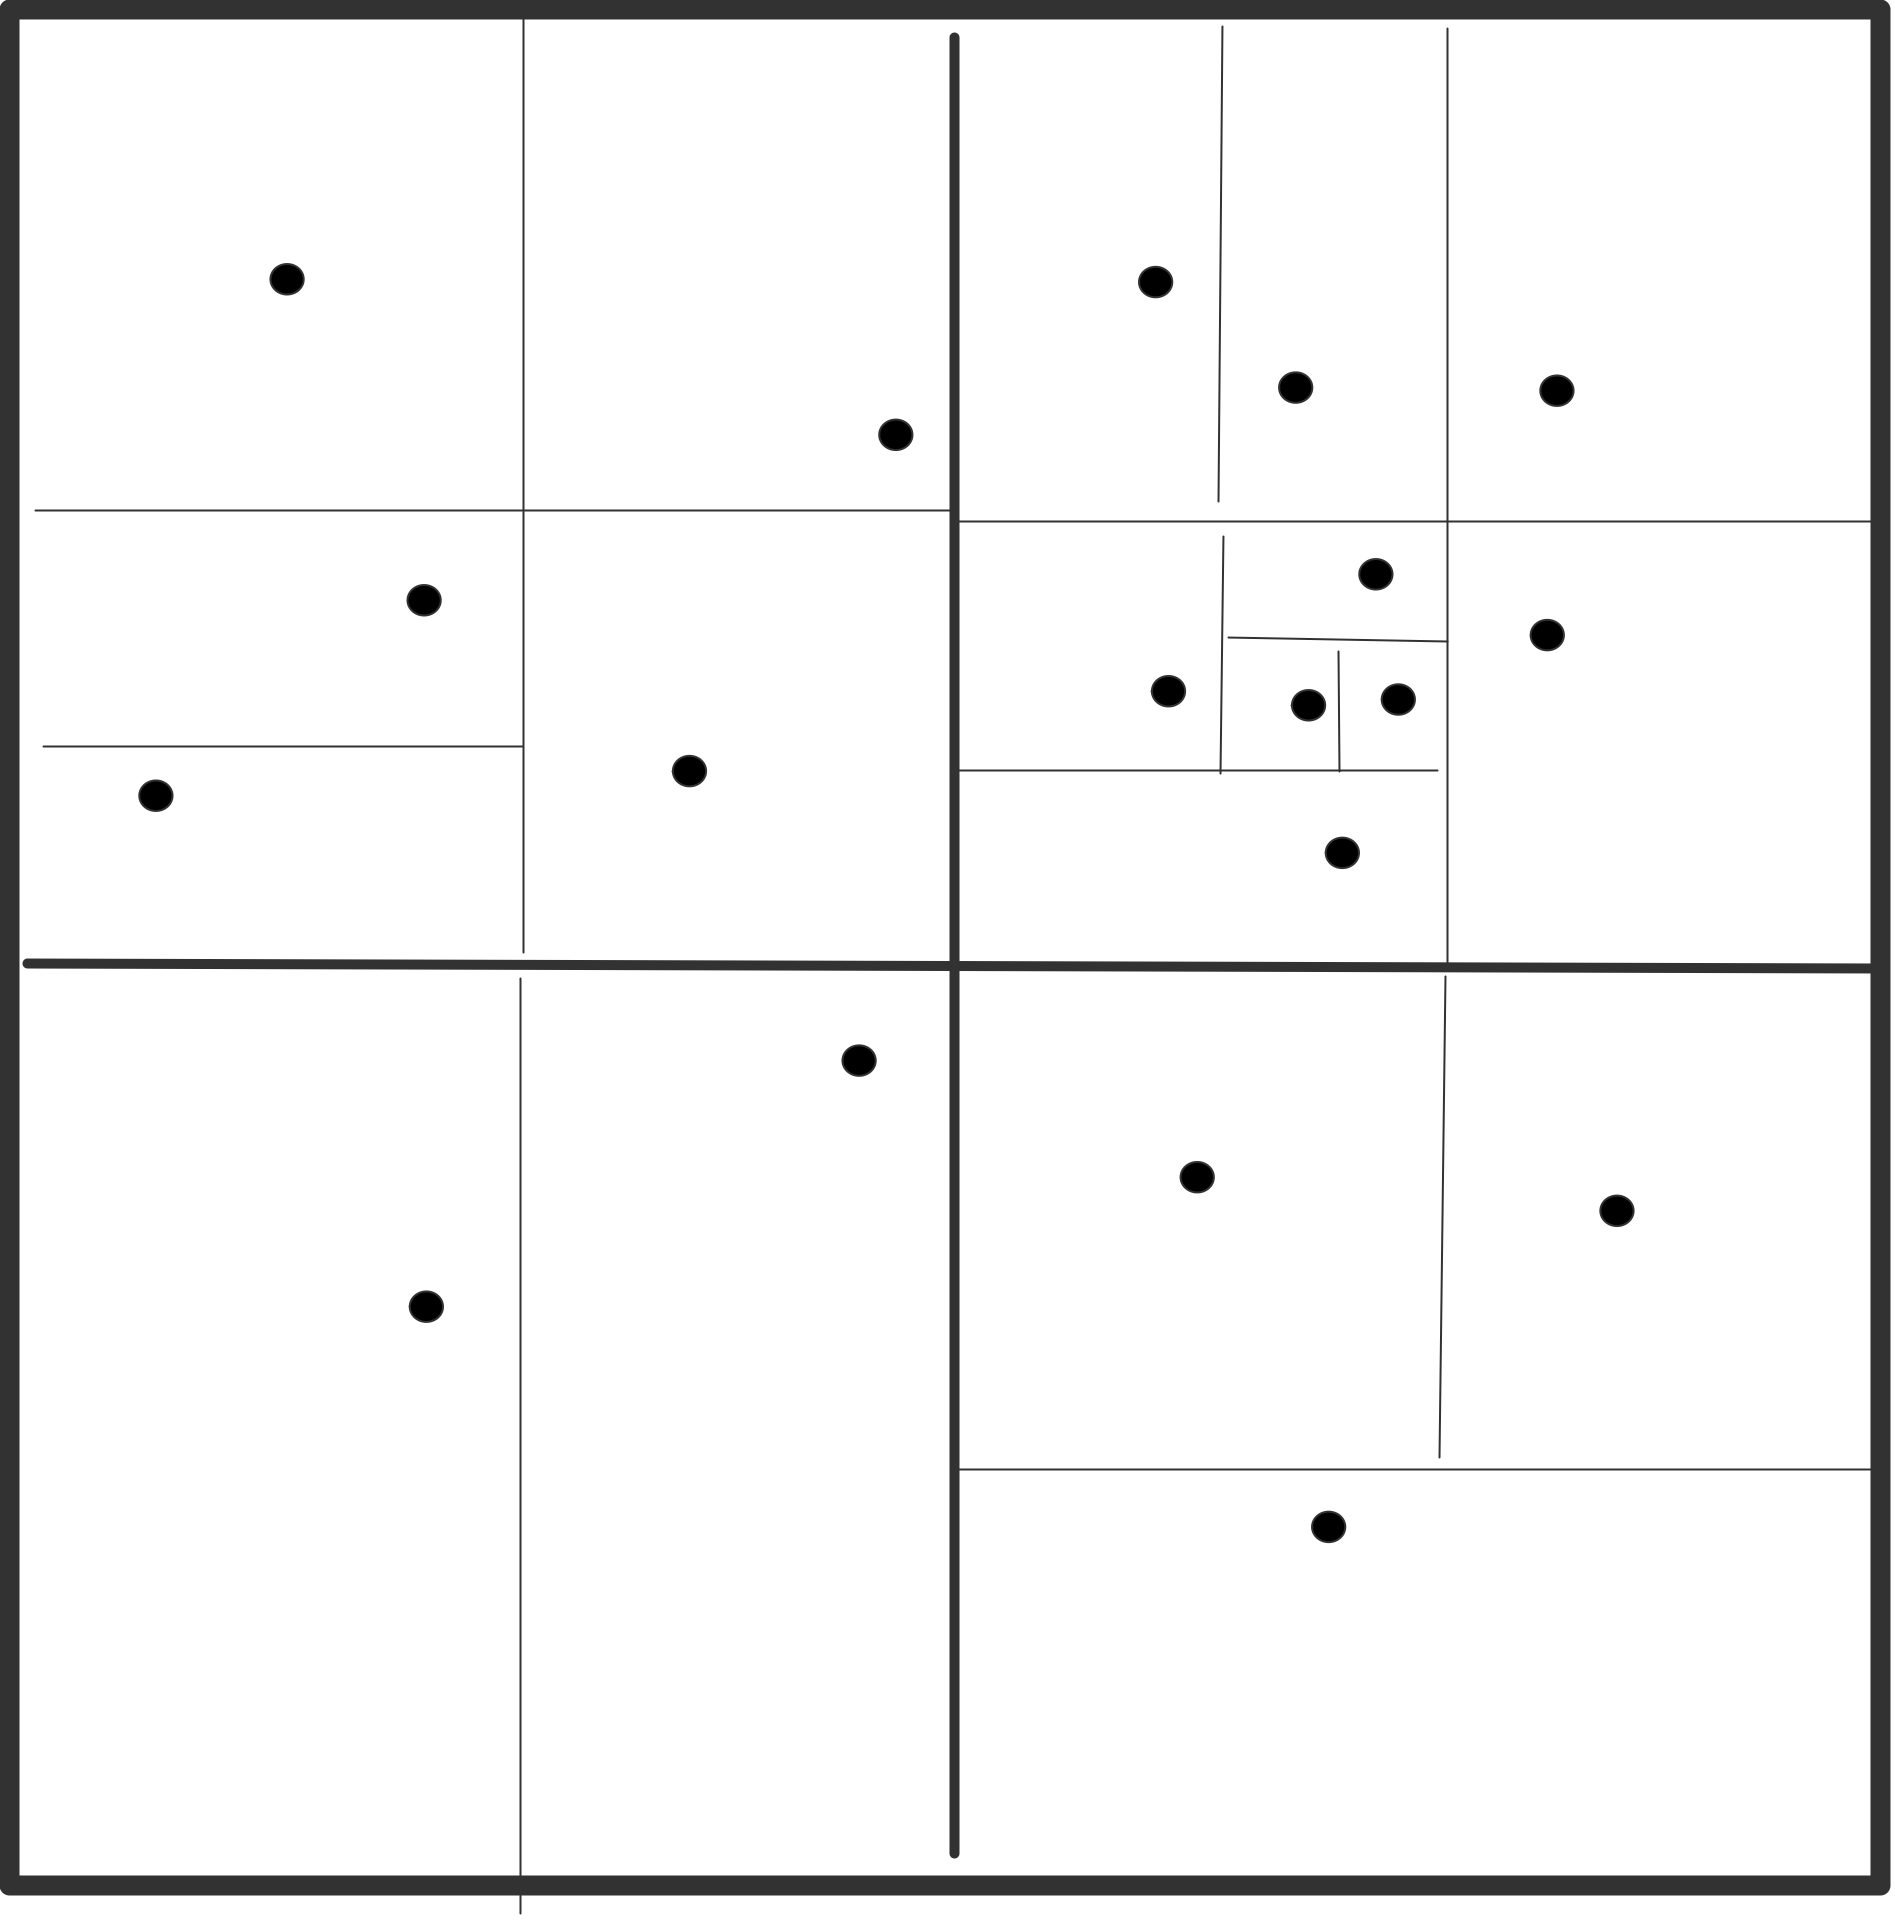
\includegraphics[scale=.05]{bh-quadrants-filled}%
  }
\end{frame}

\let\verbatimsize\footnotesize

\begin{frame}[fragile]{Dynamic octree creation}
\verbatimsize
\begin{verbatim}
Procedure Quad_Tree_Build
    Quad_Tree = {empty}
    for j = 1 to N  // loop over all N particles
         Quad_Tree_Insert(j, root)  // insert particle j in QuadTree
    endfor
    Traverse the Quad_Tree eliminating empty leaves

Procedure Quad_Tree_Insert(j, n) // Try to insert particle j at node n in Quad_Tree
    if n an internal node              // n has 4 children
        determine which child c of node n contains particle j
        Quad_Tree_Insert(j, c)
   else if n contains 1 particle   //  n is a leaf
        add n's 4 children to the Quad_Tree
        move the particle already in n into the child containing it
        let c be the child of n containing j
        Quad_Tree_Insert(j, c)
    else                                         //  n empty 
        store particle j in node n
    end
\end{verbatim}
\end{frame}

\begin{frame}{Octree algorithm}
  \begin{itemize}
  \item Consider cells on the top level
  \item if distance/diameter ratio small enough, take center of mass
  \item otherwise consider children cells
  \end{itemize}
\end{frame}

\begin{frame}
  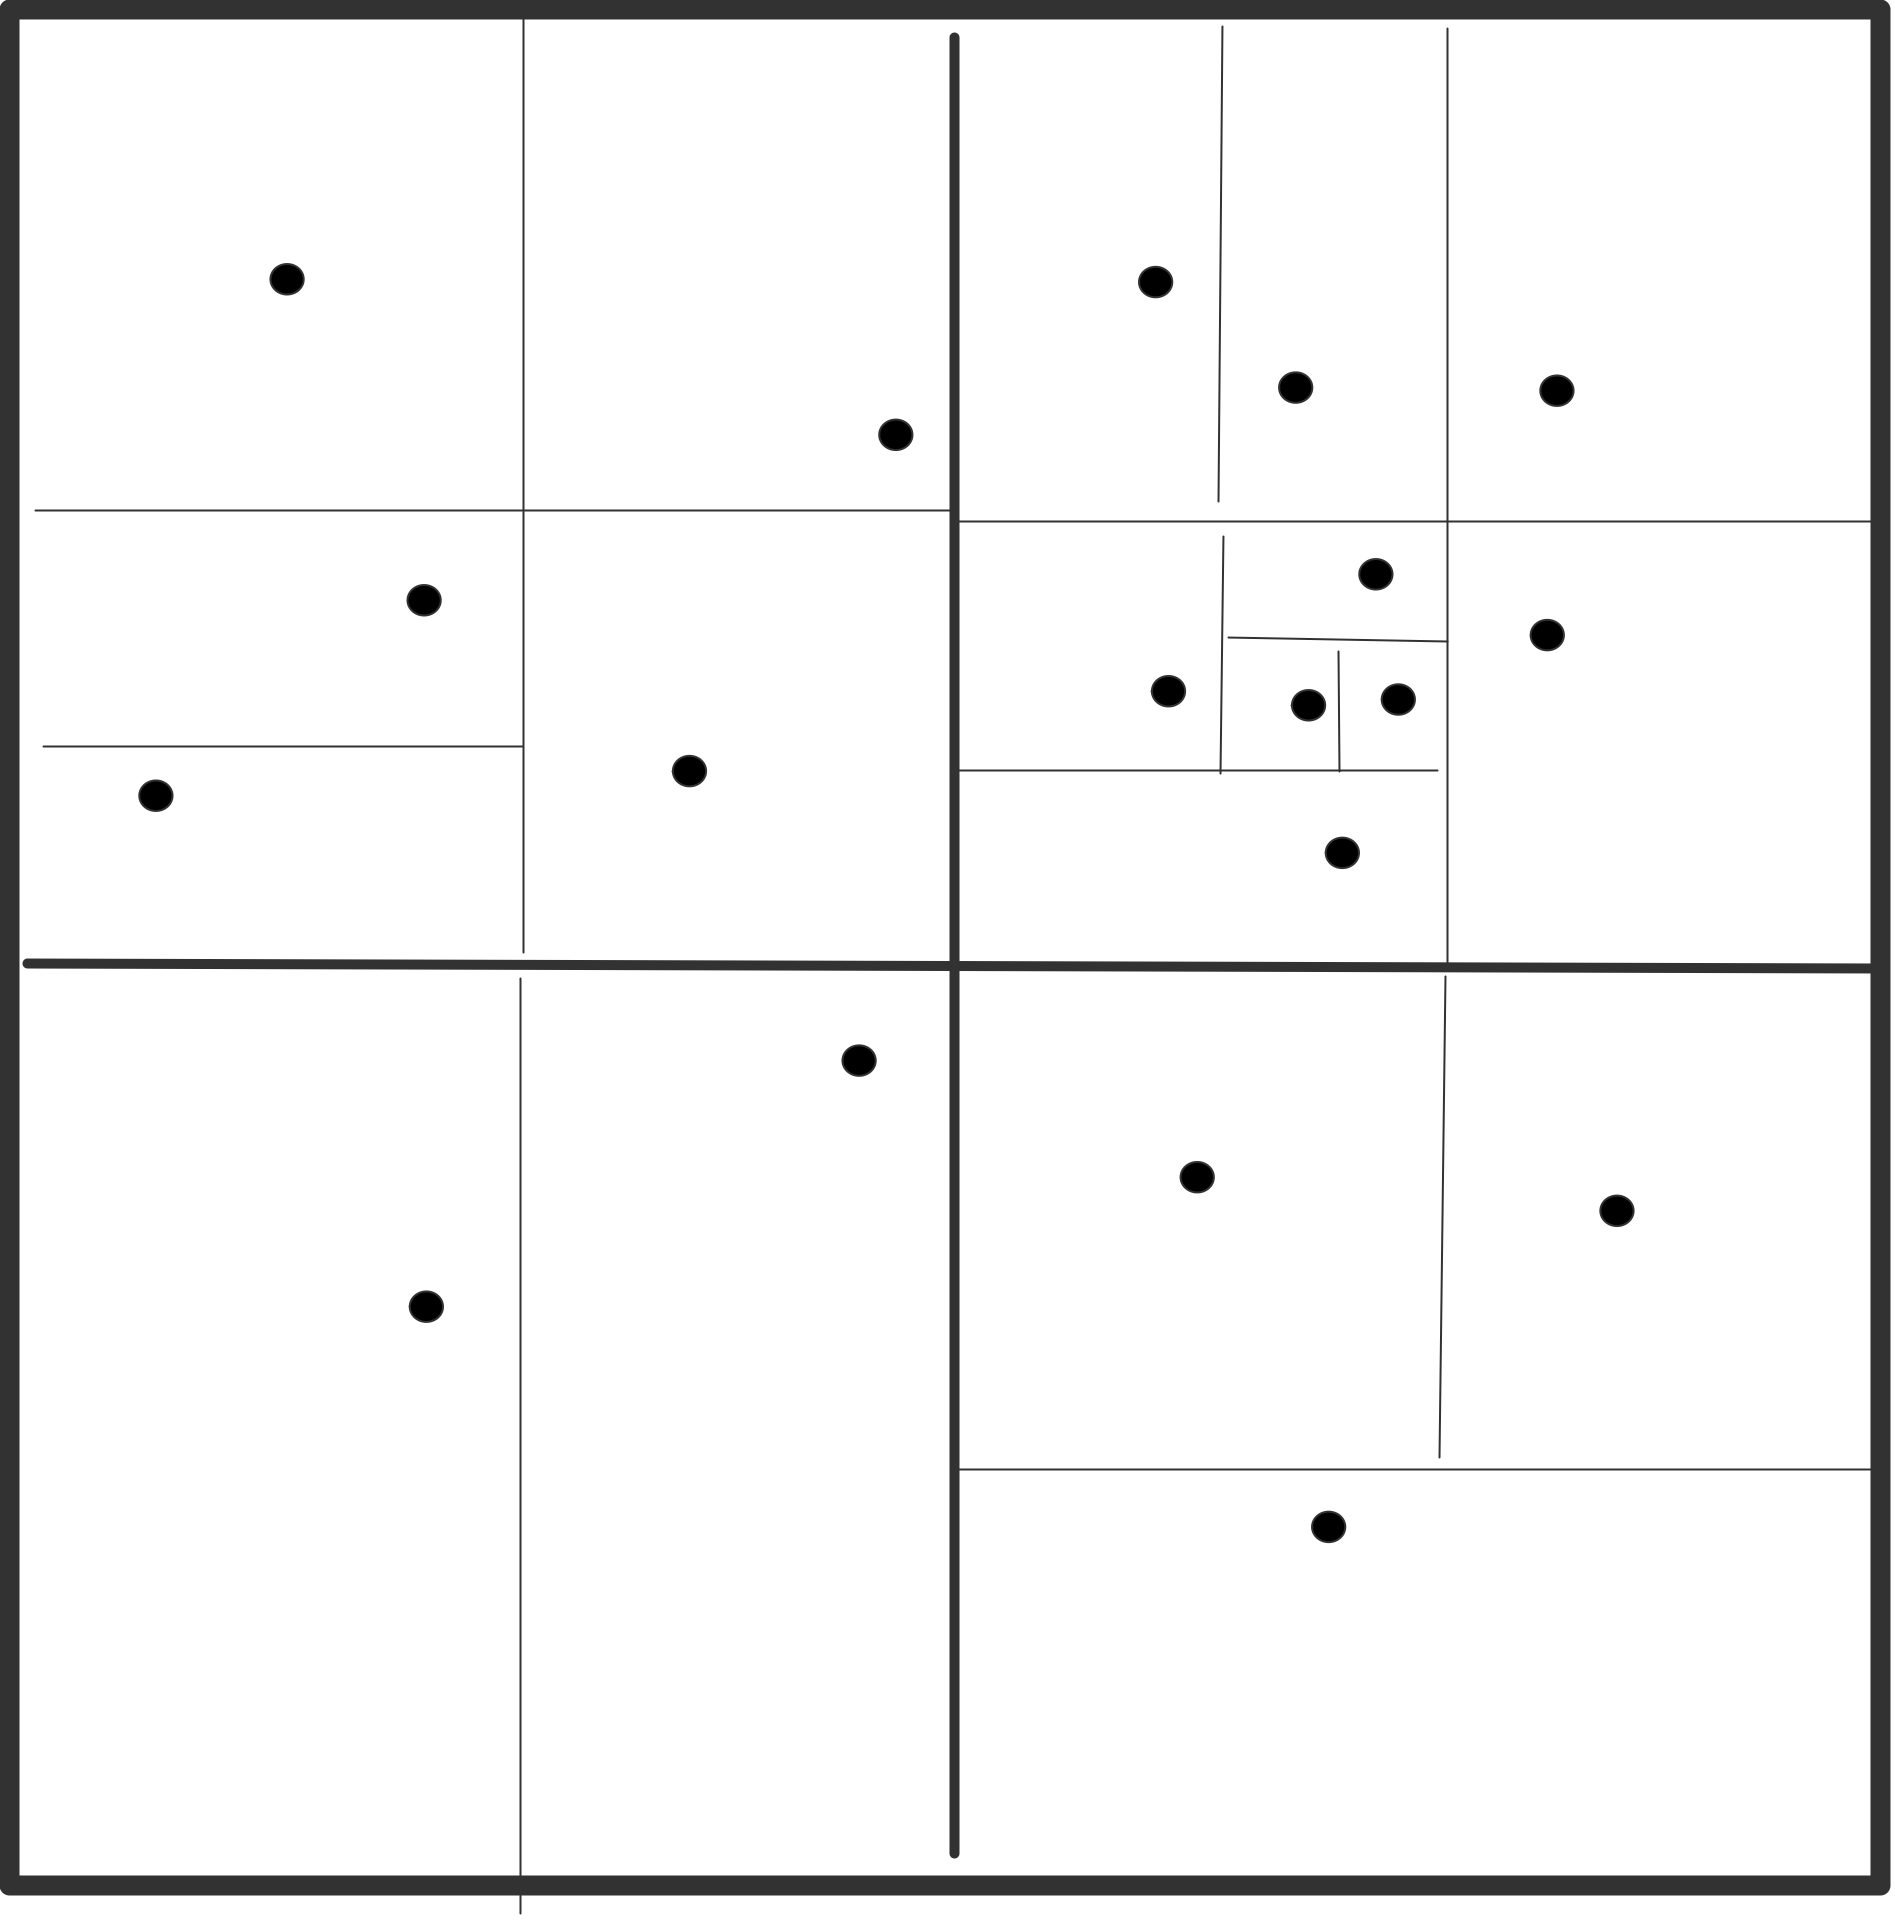
\includegraphics[scale=.08]{bh-quadrants-filled}
  %
  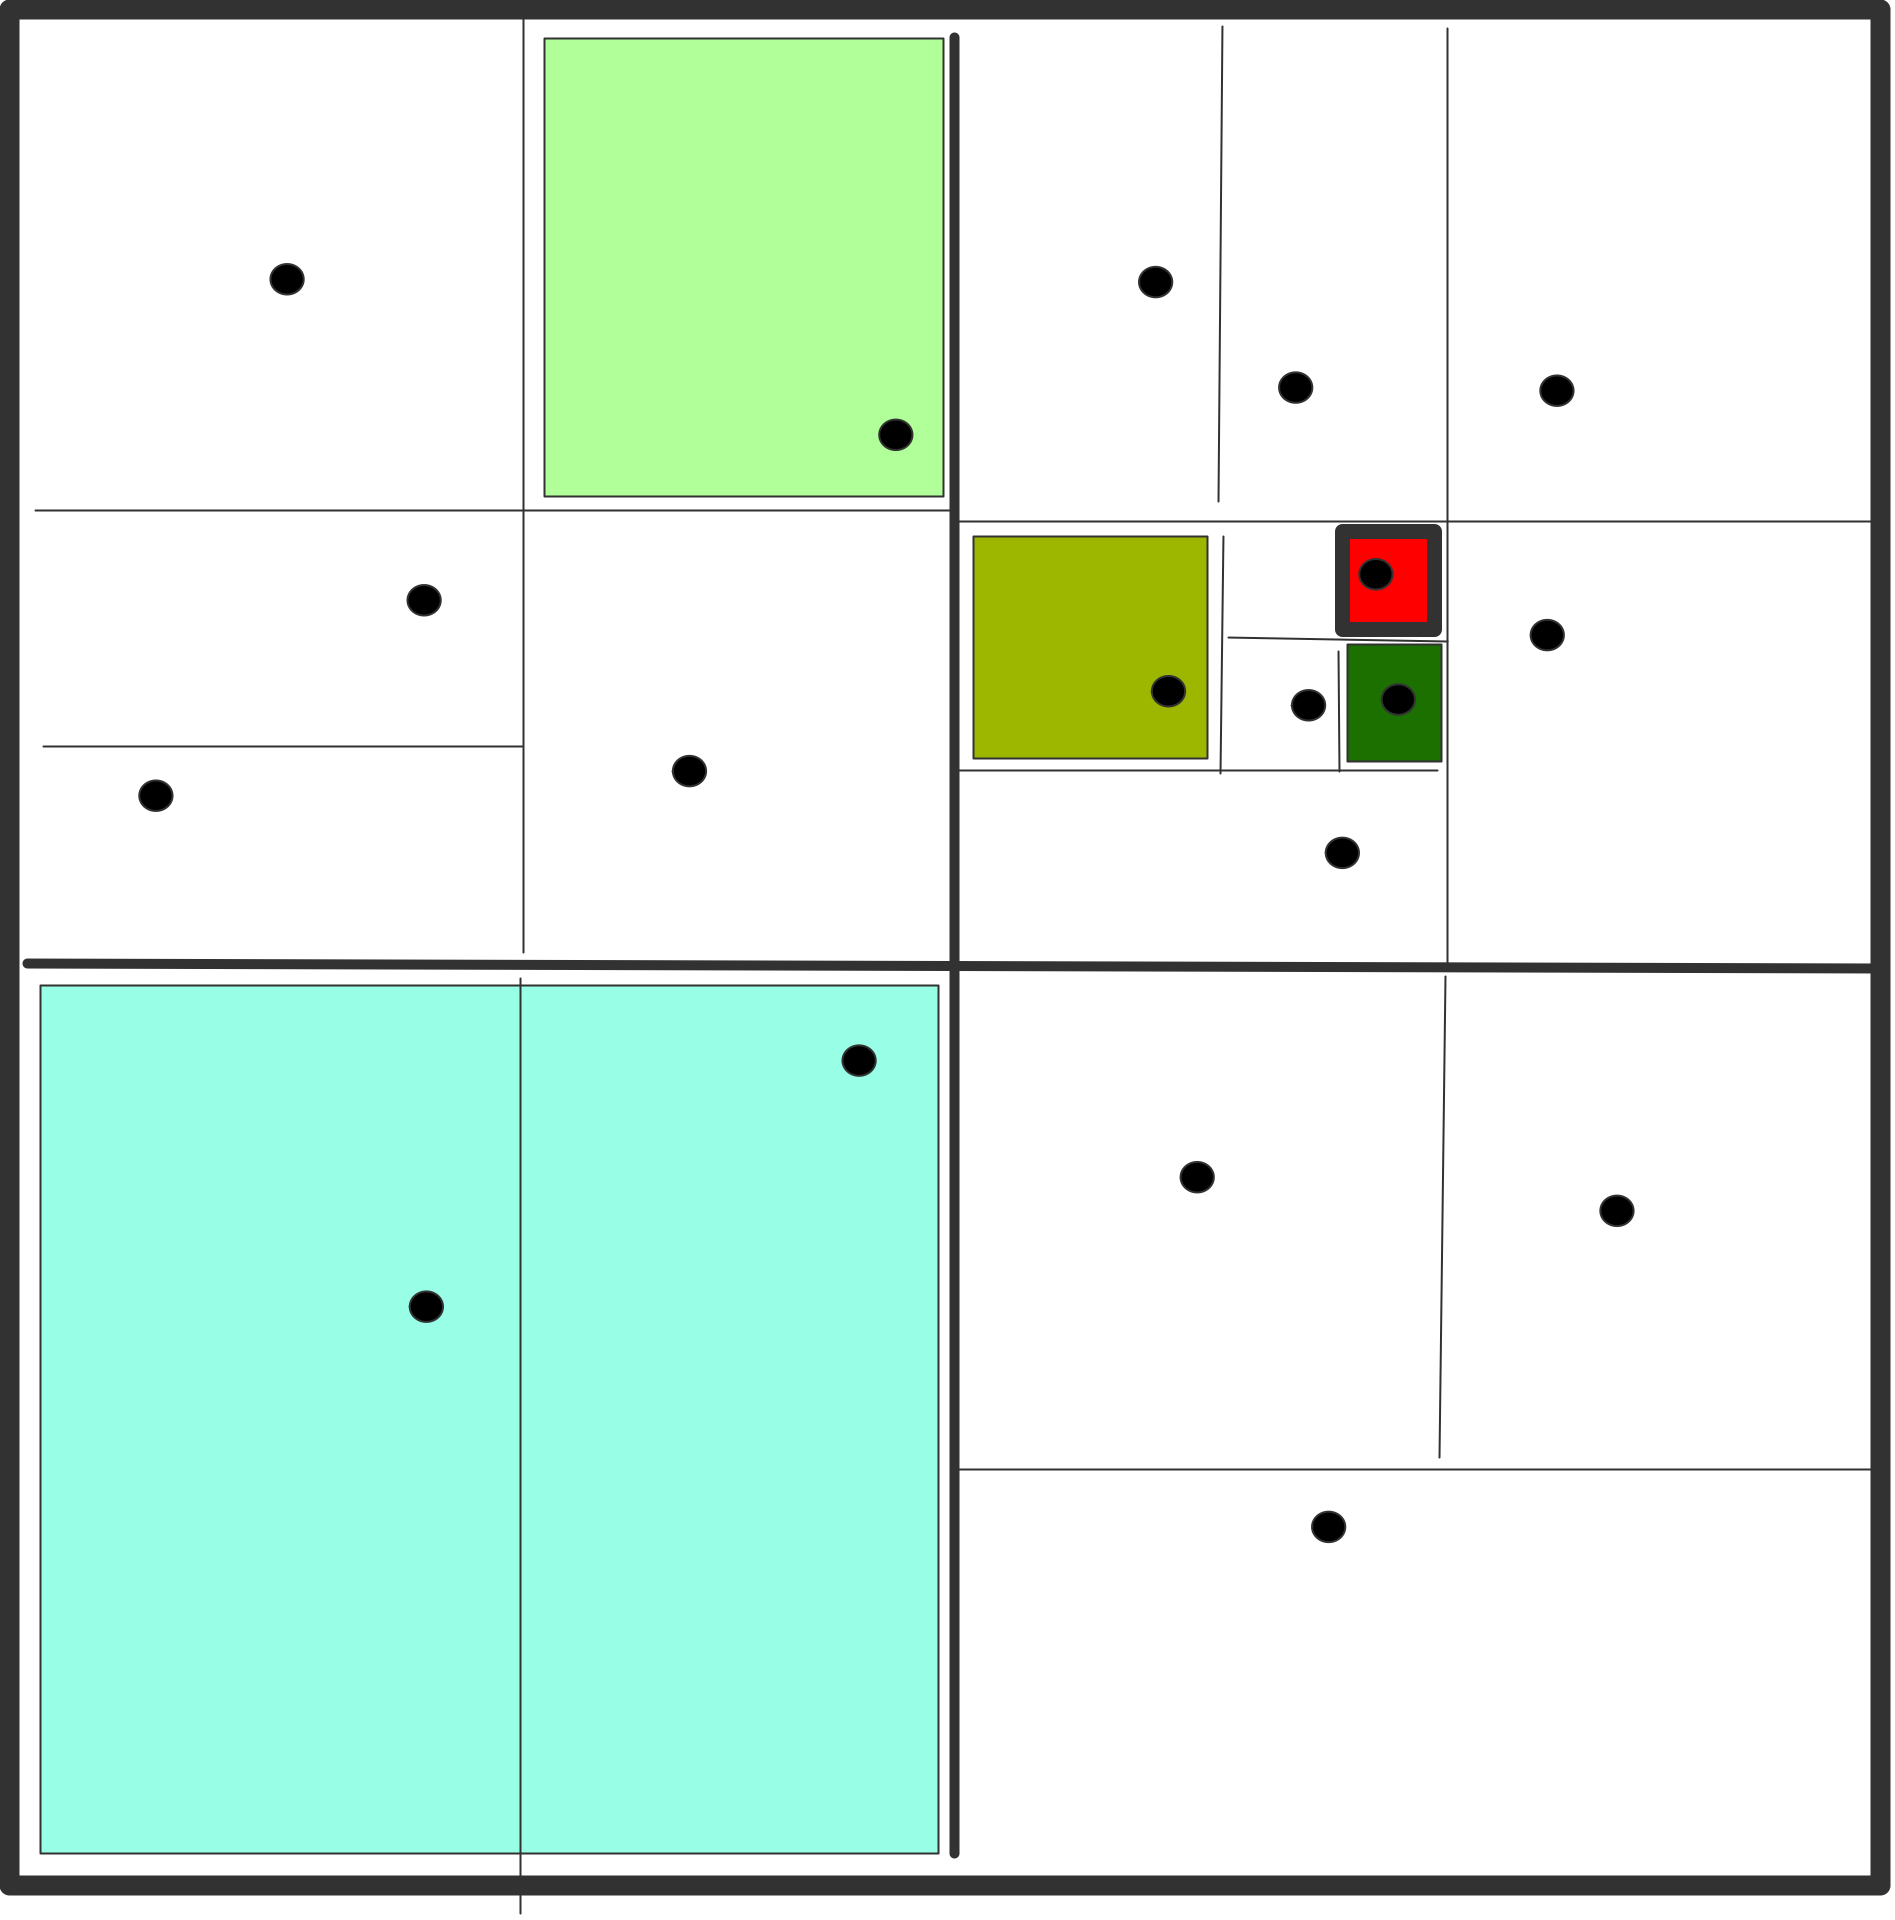
\includegraphics[scale=.08]{bh-quadrants-ratio}
\end{frame}

\begin{frame}[fragile]{Masses calculation}
\verbatimsize
\begin{verbatim}
// Compute the CM = Center of Mass and TM = Total Mass of all the particles 
( TM, CM ) = Compute_Mass( root )

function ( TM, CM ) = Compute_Mass( n )
  if n contains 1 particle
     store (TM, CM) at n
     return (TM, CM)
  else       // post order traversal
             // process parent after all children
     for all children c(j) of n
           ( TM(j), CM(j) ) = Compute_Mass( c(j) )
     // total mass is the sum
     TM = sum over children j of n: TM(j)
     // center of mass is weighted sum
     CM = sum over children j of n: TM(j)*CM(j) / TM
     store ( TM, CM ) at n
     return ( TM, CM )
\end{verbatim}
\end{frame}

\begin{frame}[fragile]{Force evaluation}
\verbatimsize
\begin{verbatim}
// for each particle, compute the force on it by tree traversal
for k = 1 to N
    f(k) = TreeForce( k, root )   
    // compute force on particle k due to all particles inside root

function f = TreeForce( k, n )   
    // compute force on particle k due to all particles inside node n
    f = 0
    if n contains one particle  // evaluate directly
        f = force computed using formula on last slide
    else
        r = distance from particle k to CM of particles in n
        D = size of n
        if  D/r  < theta  // ok to approximate by CM and TM
             compute f 
        else              // need to look inside node
             for all children c of n
                   f = f + TreeForce ( k, c )
\end{verbatim}
\end{frame}

\begin{frame}{Complexity}
  \begin{itemize}
  \item Each cell considers `rings' of equi-distant cells
  \item but at doubling distance
  \item $c\log N$ cells to consider for each particle
  \item $N\log N$ overall
  \end{itemize}  
\end{frame}

\begin{frame}{Computational aspects}
  \begin{itemize}
  \item After position update, particles can move to next box: load redistribution
  \item Naive octree algorithm is formulated for shared memory
  \item Distributed memory by using inspector-executor paradigm
  \end{itemize}
\end{frame}

\begin{frame}{Step 1: force by a particle}
  \begin{tabbing}
    for \=level $\ell$ from one above the finest to the coarsest:\\
    \>for \=each cell $c$ on level $\ell$\\
    \>\>let $g^{(\ell)}_c$ be the \=combination of the $g^{(\ell+1)}_i$
    for all children $i$ of $c$
  \end{tabbing}
\end{frame}

\begin{frame}
  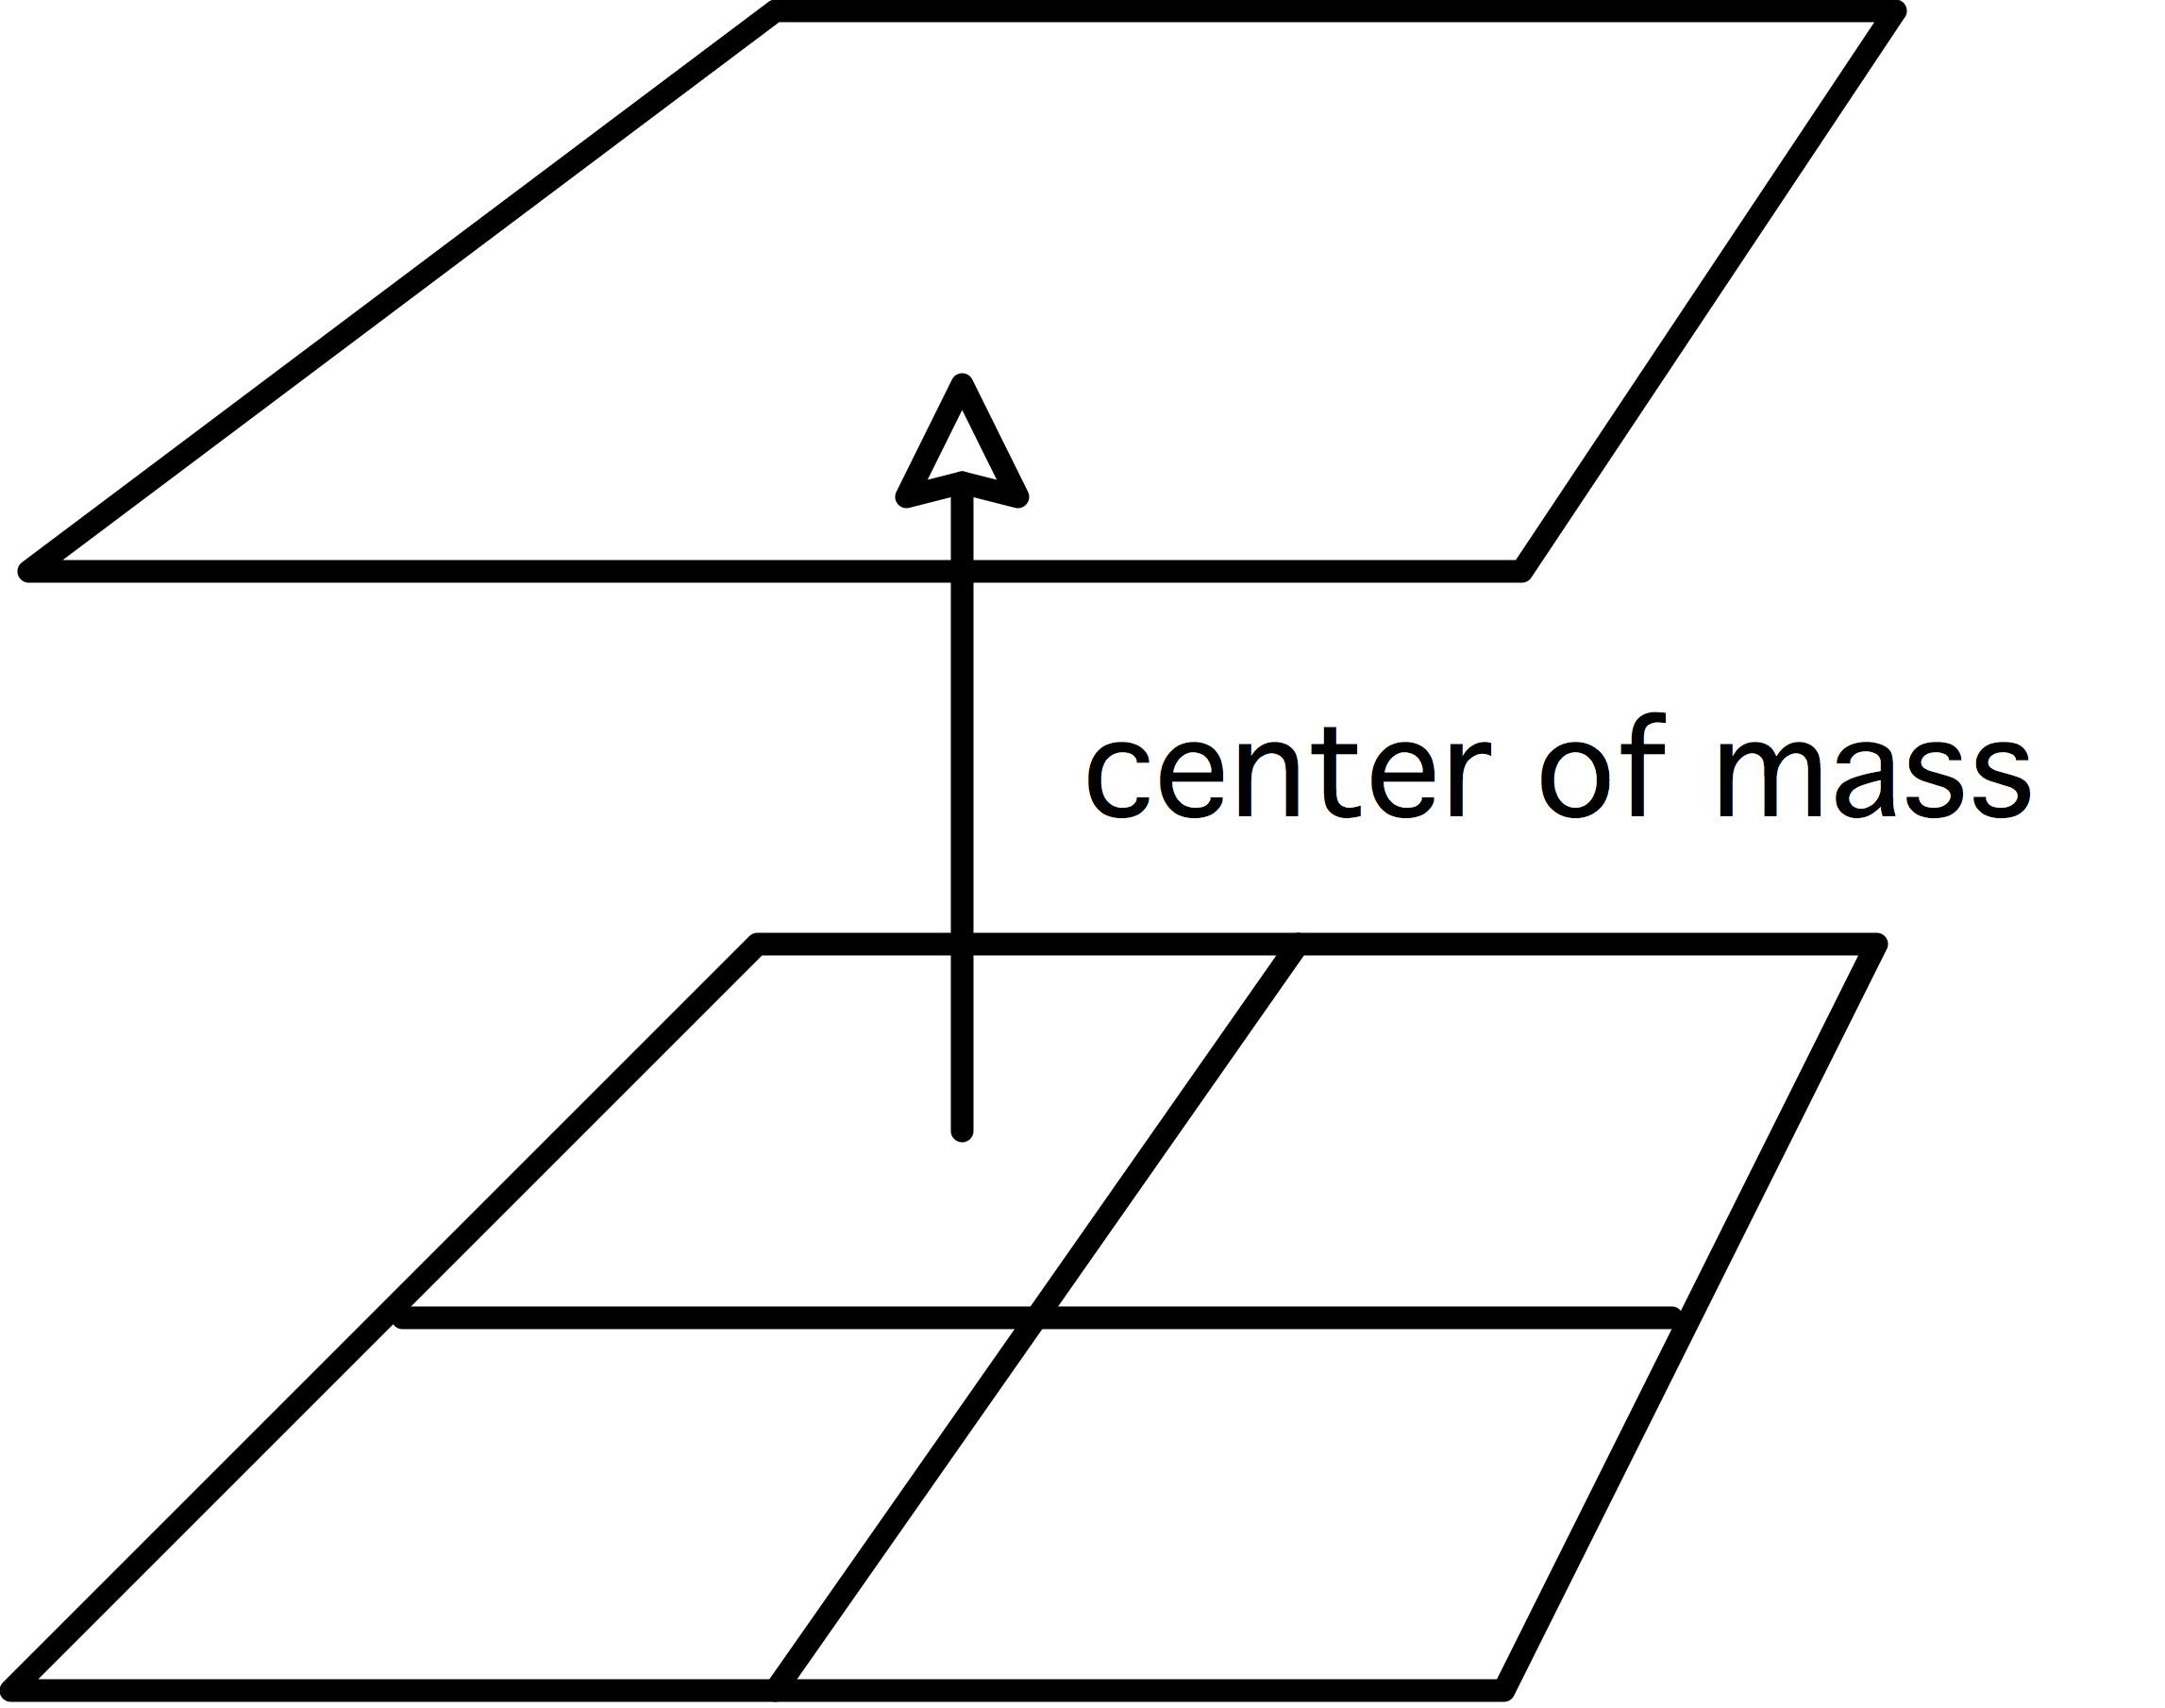
\includegraphics[scale=.1]{bh-up}
\end{frame}

\begin{frame}{Step 2: force on a particle}
  \begin{tabbing}
    for \=level $\ell$ from one below the coarses to the finest:\\
    \>for \=each cell $c$ on level $\ell$:\\
    \>\>let $f^{(\ell)}_c$ \=be the sum of\\
    \>\>\>1. the force $f^{(\ell-1)}_p$ on the parent $p$ of $c$, and\\
    \>\>\>2. the sums $g^{(\ell)}_i$ for \=all $i$ on level $\ell$ that\\
    \>\>\>\>satisfy the cell opening criterium
  \end{tabbing}
\end{frame}

\begin{frame}
  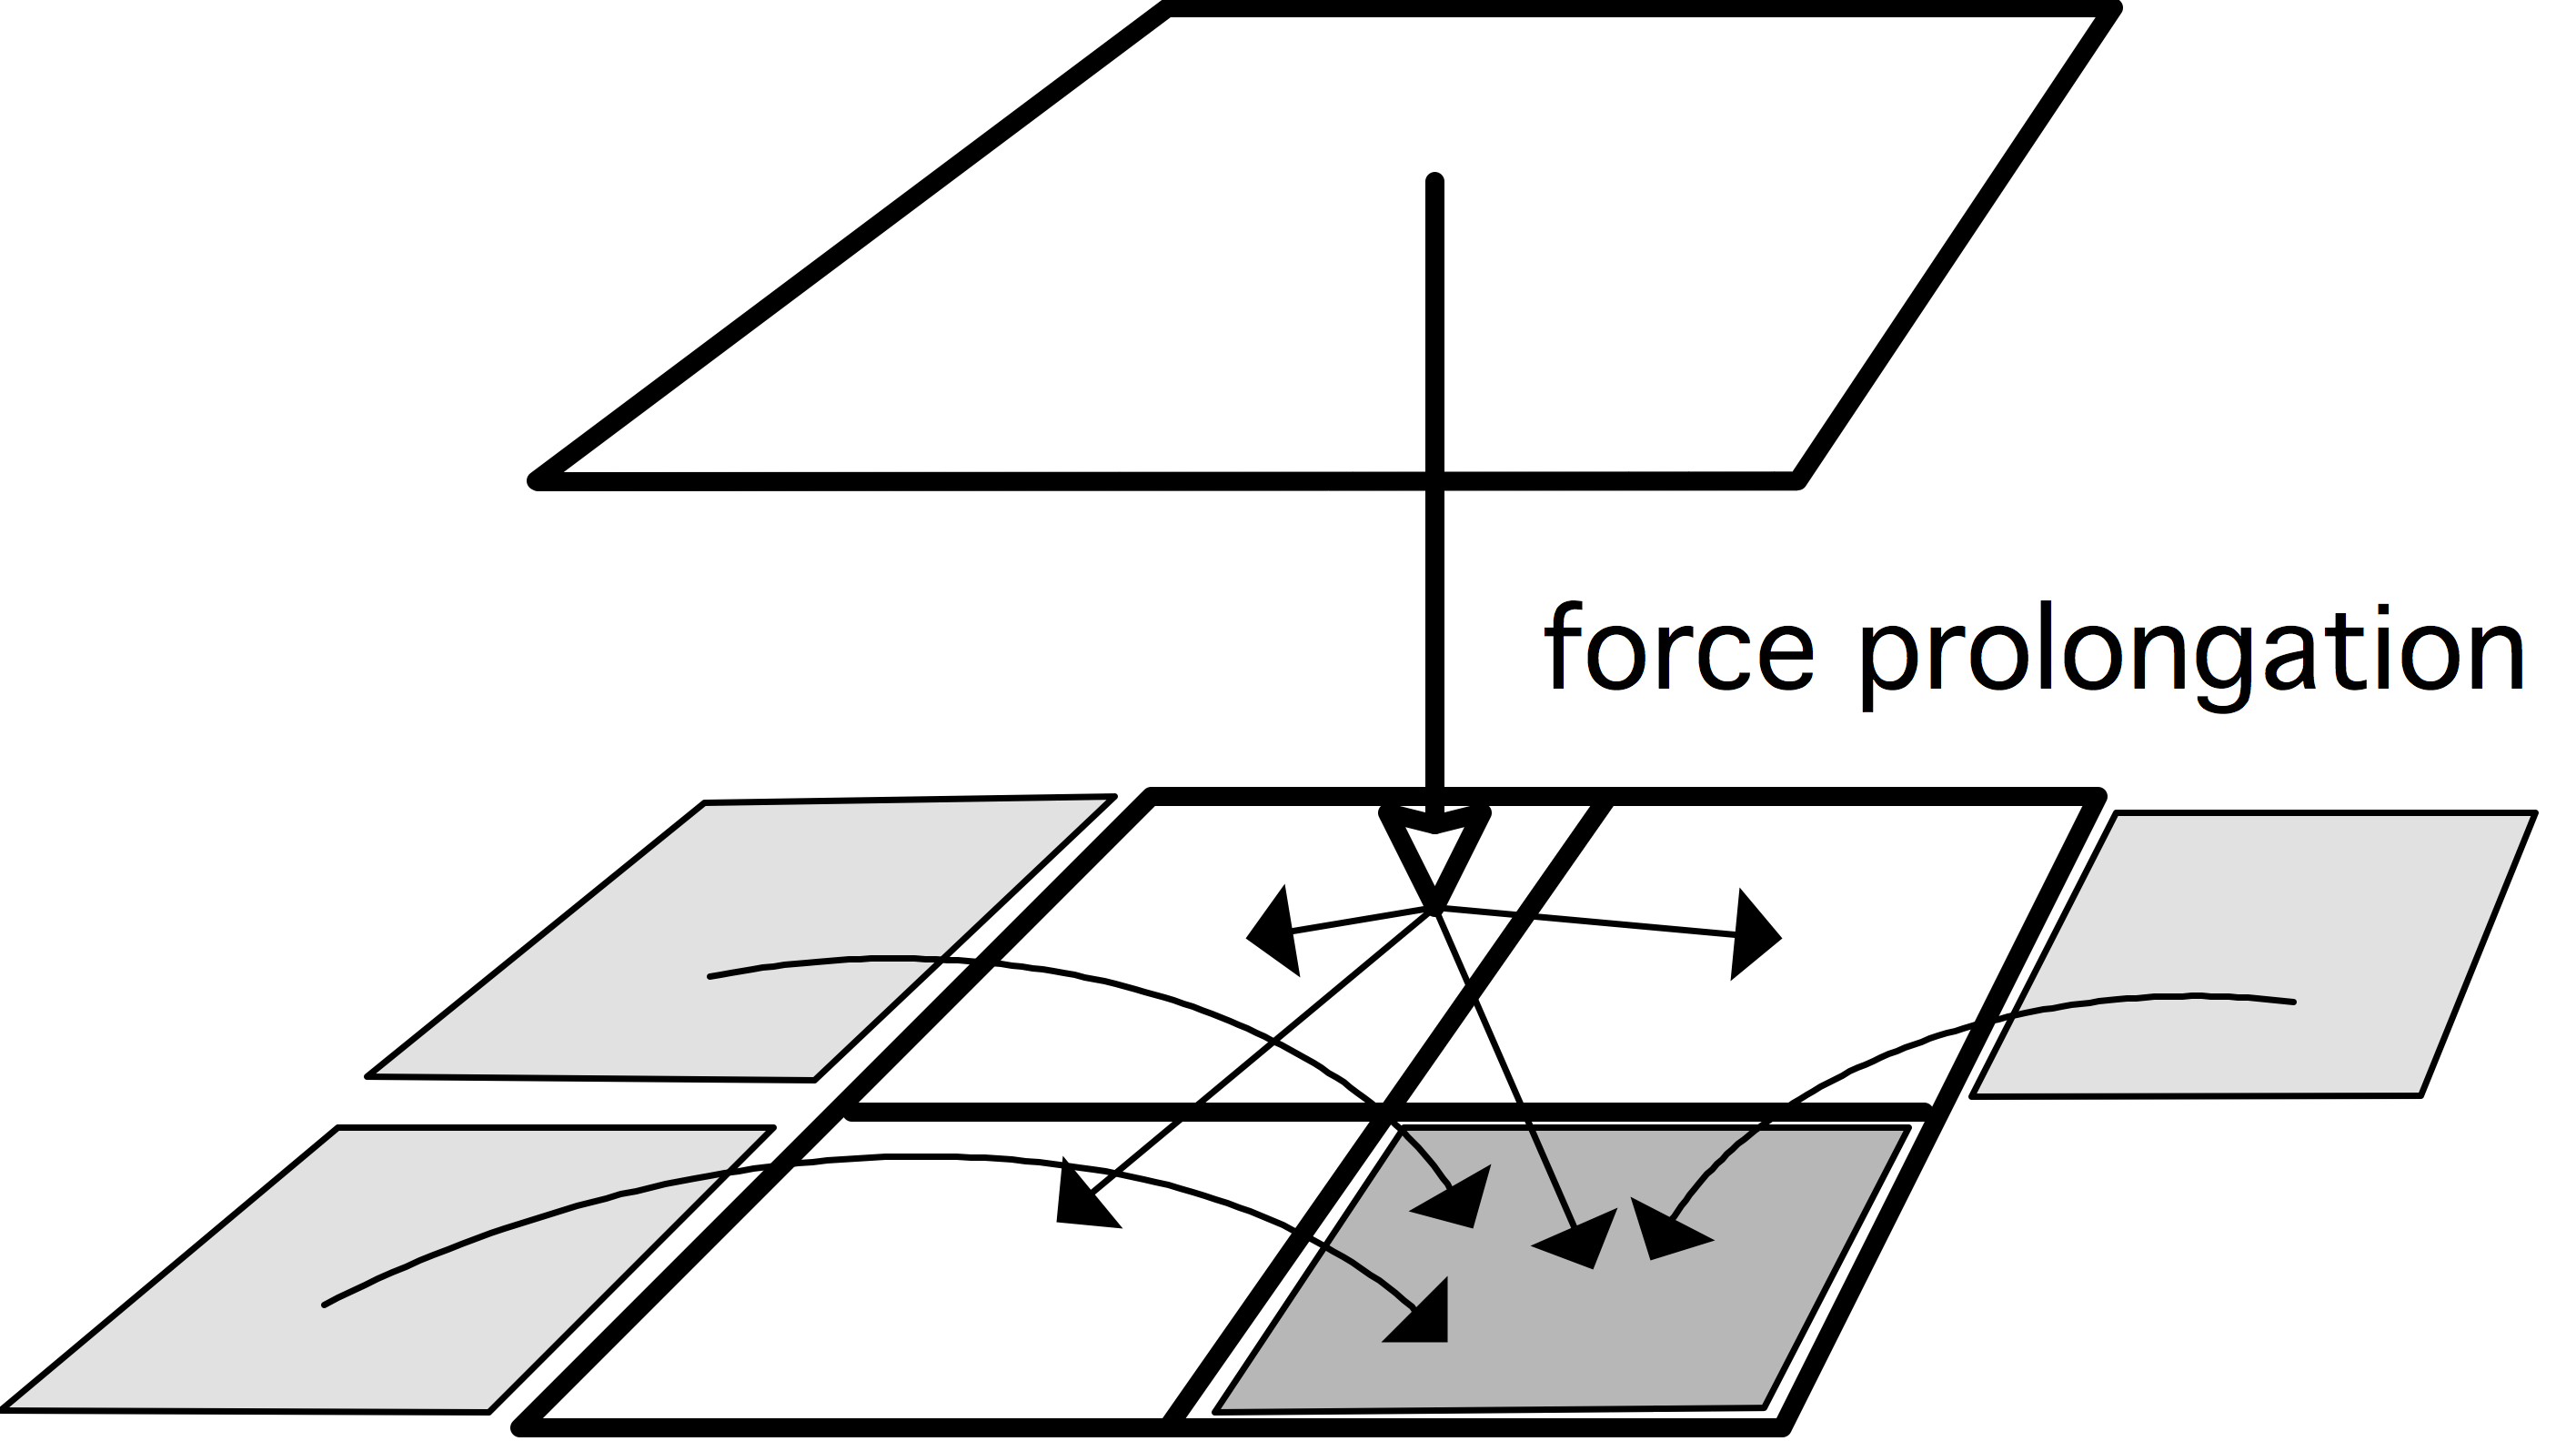
\includegraphics[scale=.1]{bh-down}
\end{frame}

\begin{frame}
  \begin{itemize}
  \item Center of mass calculation and force prolongation are local
  \item Force from neighbouring cells is a neighbour communication
  \item Neighbour communication can start before up/down tree
    calculation is finished: latency hiding
  \end{itemize}
\end{frame}

\begin{frame}{All-pairs methods}
  \begin{itemize}
  \item Traditional algorithm: distribute particles,
    for each particle gather and update compute
  \item Problem: allgather has $O(N)\beta$ cost
  \item does not go down with~$P$, so does not scale weakly
  \end{itemize}
\end{frame}

\begin{frame}{1.5D calculation}
  \begin{itemize}
  \item Better algorithm: use $\sqrt P\times\sqrt P$ processor grid,
  \item Divide particles in bins of $N/\sqrt P$
  \item Processor $(i,j)$ computes interaction of boxes $i$ and~$j$:
  \end{itemize}
\end{frame}

%% \begin{frame}
%%   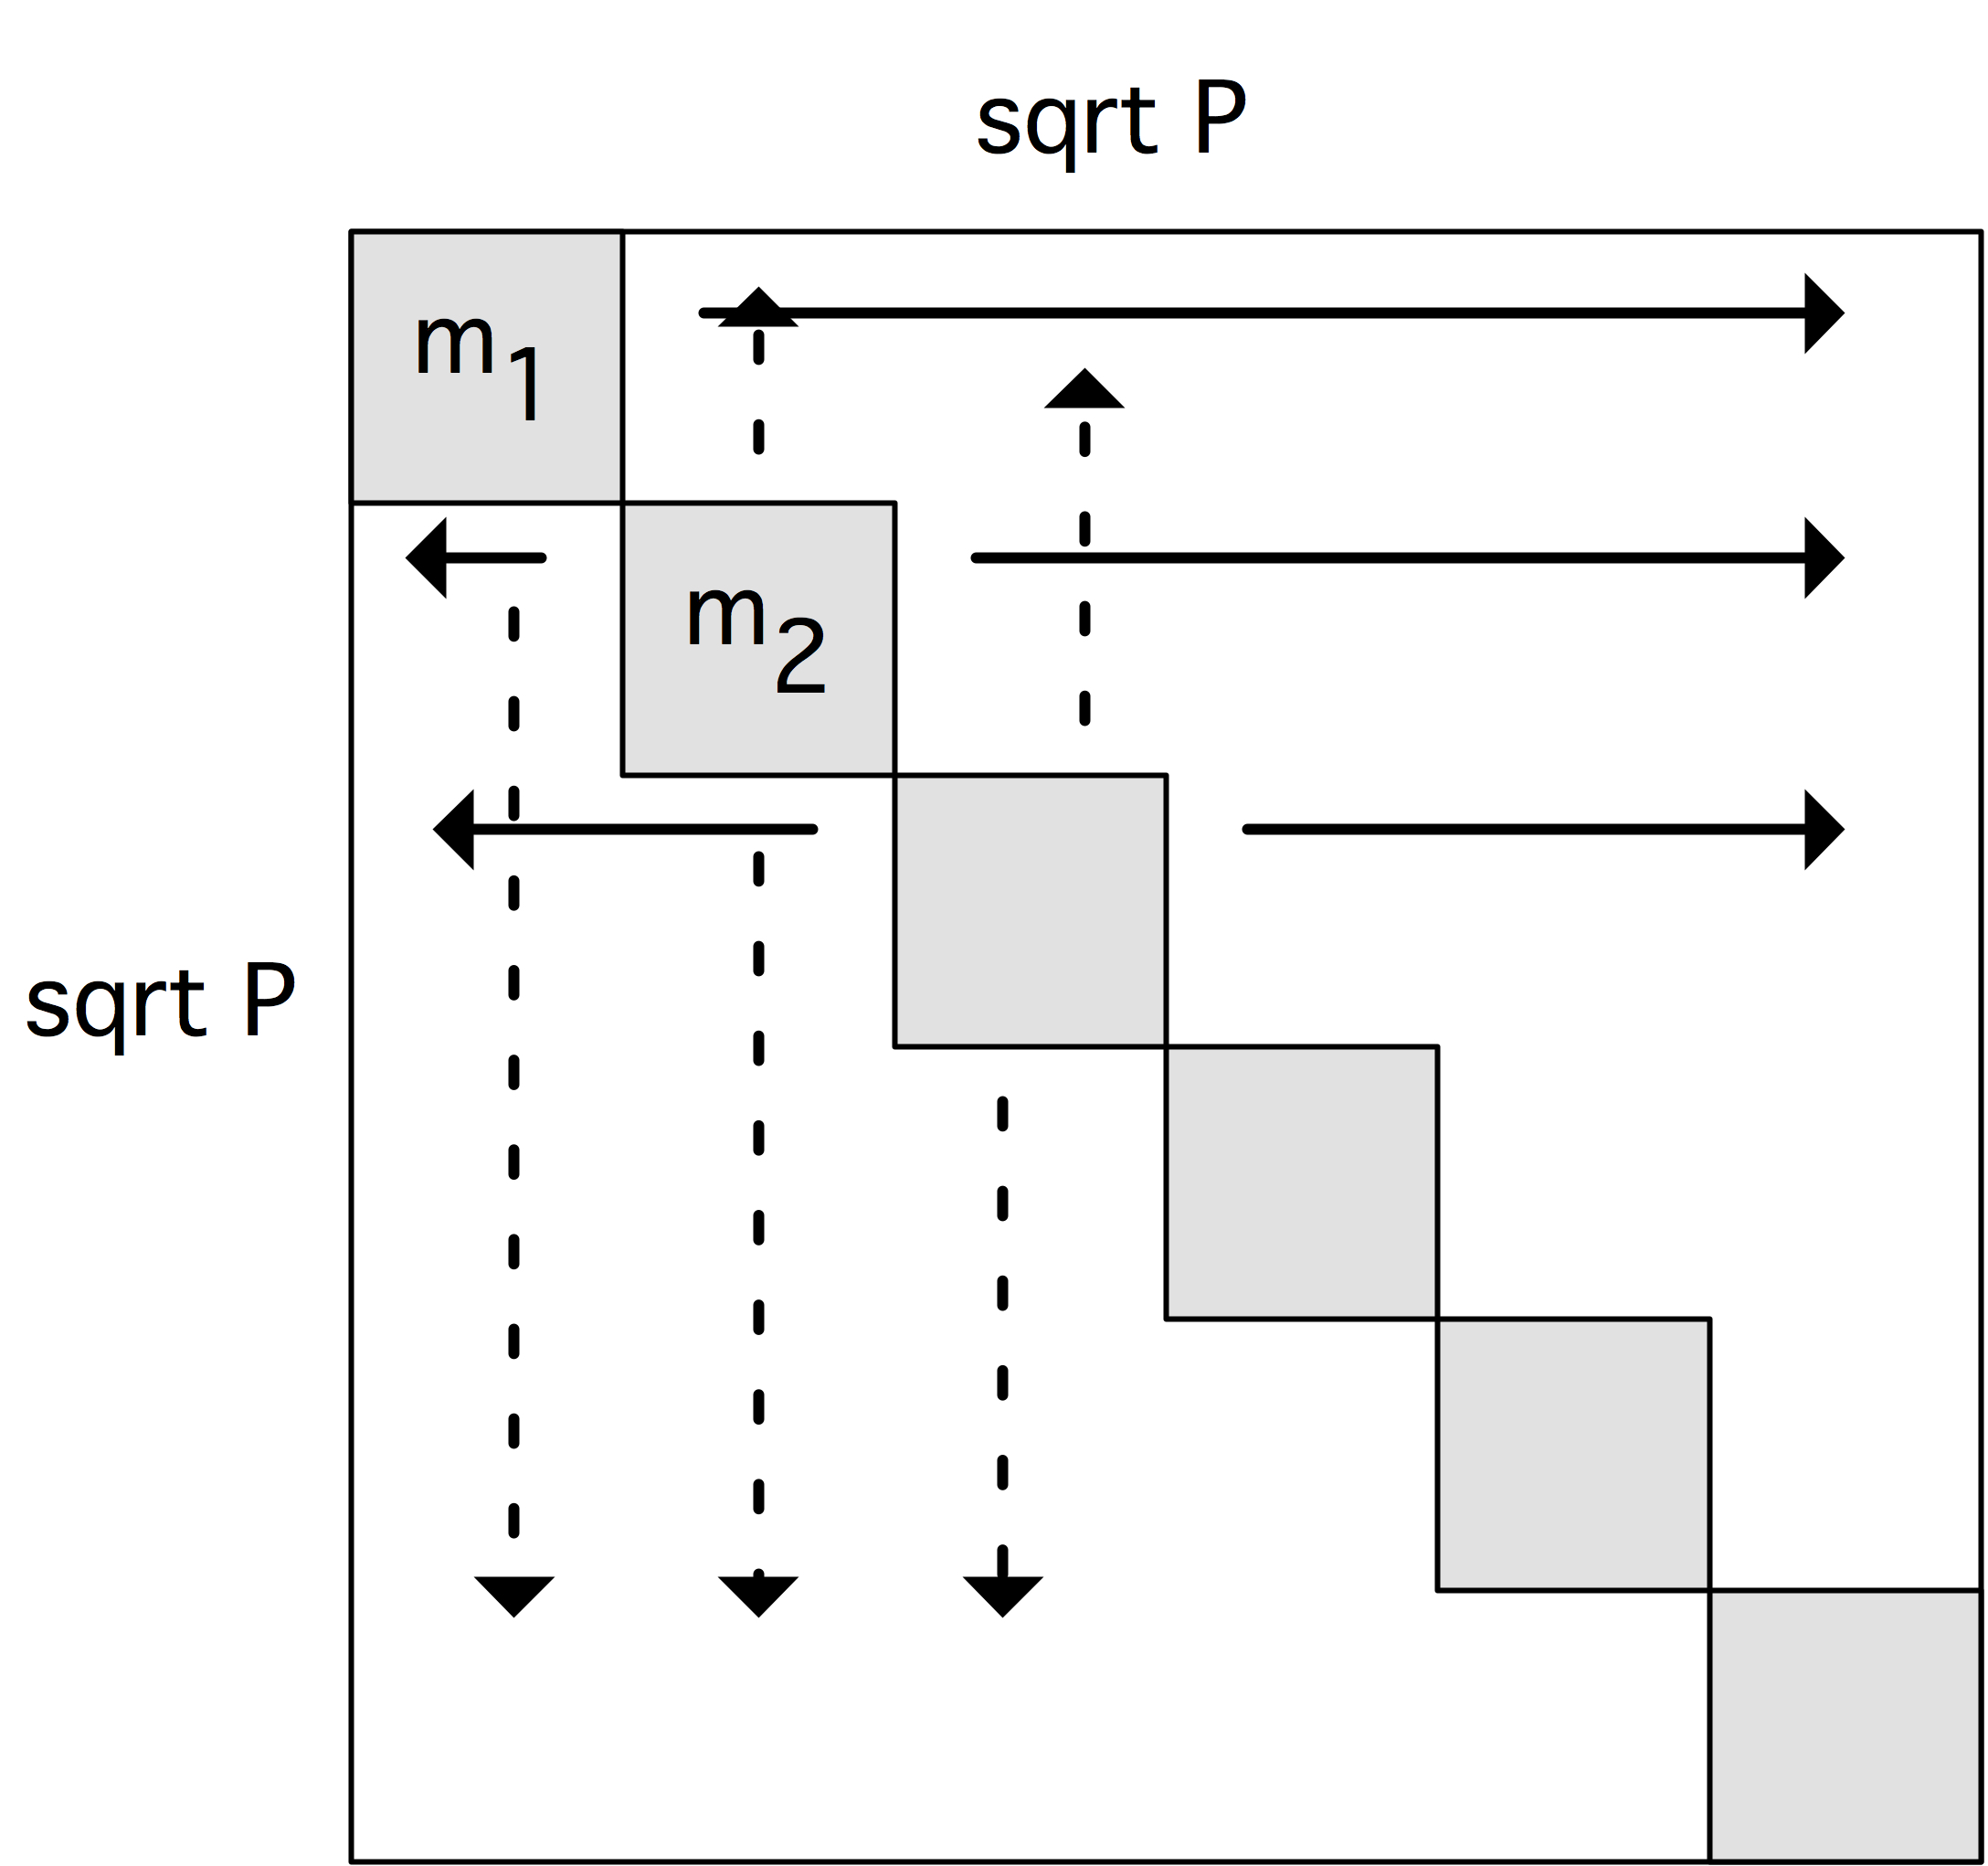
\includegraphics[scale=.1]{all-pairs}
%% \end{frame}

\begin{frame}
  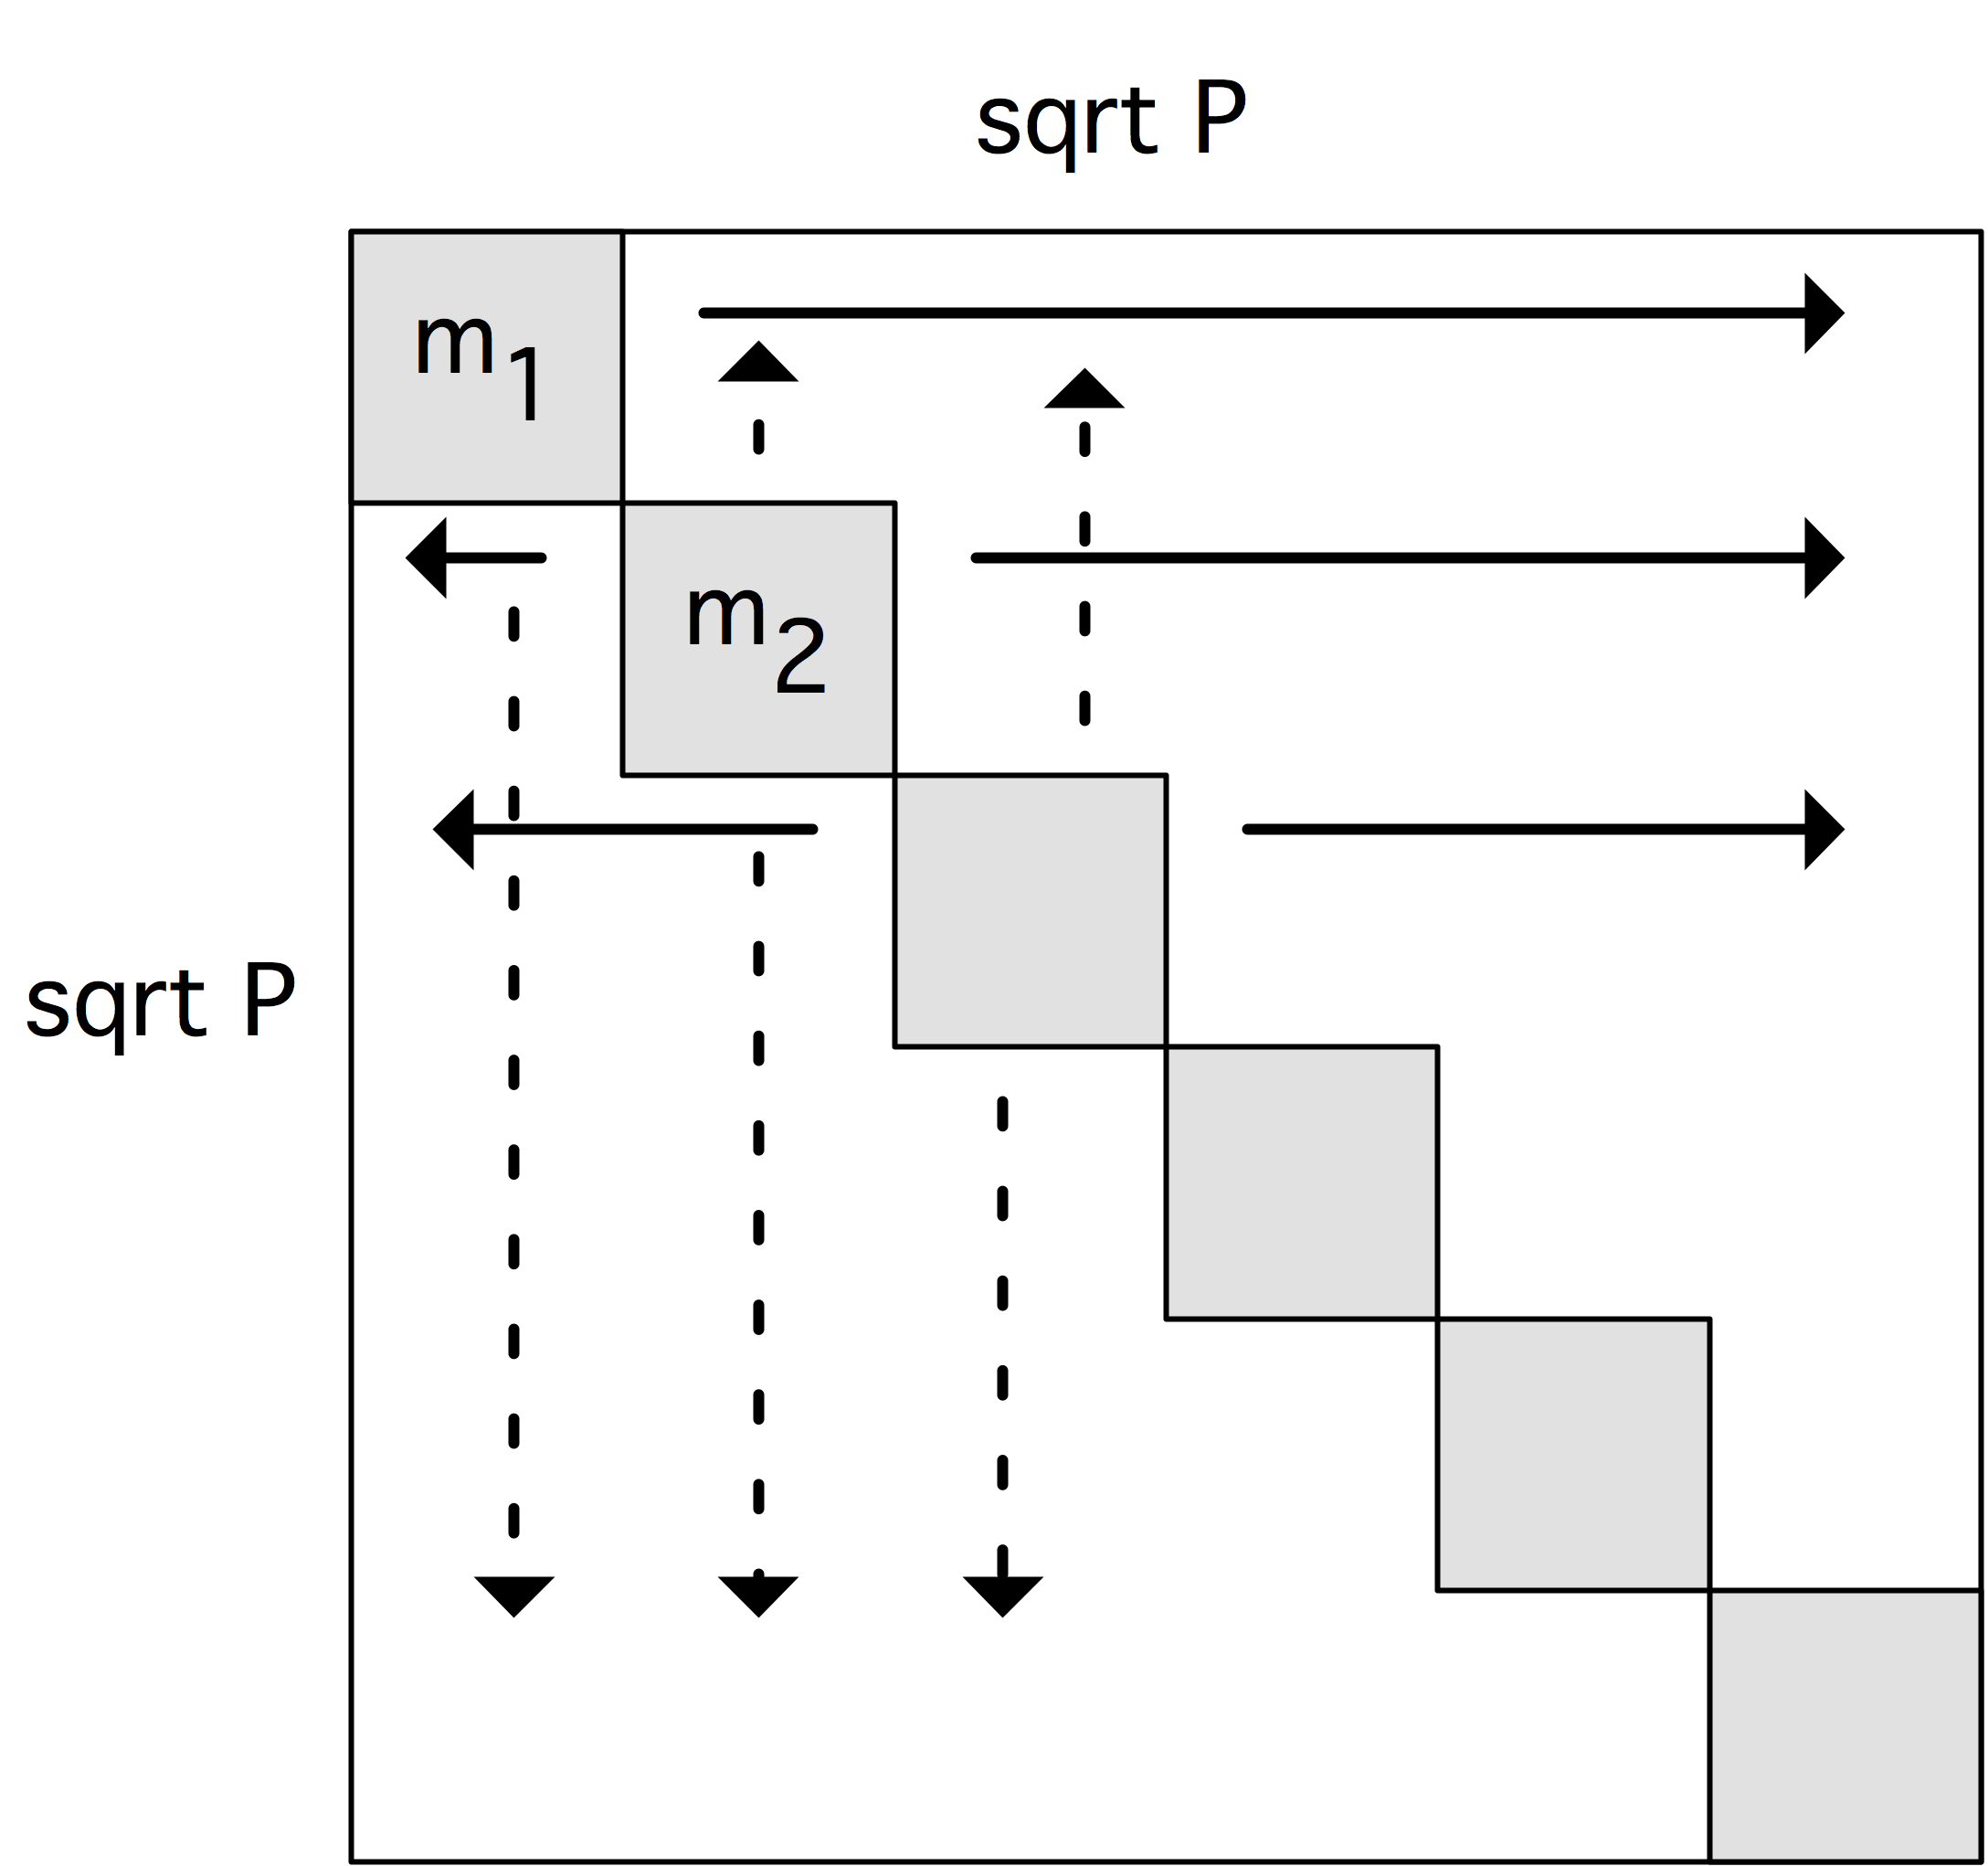
\includegraphics[scale=.1]{all-pairs-bcst}
\end{frame}

\begin{frame}
  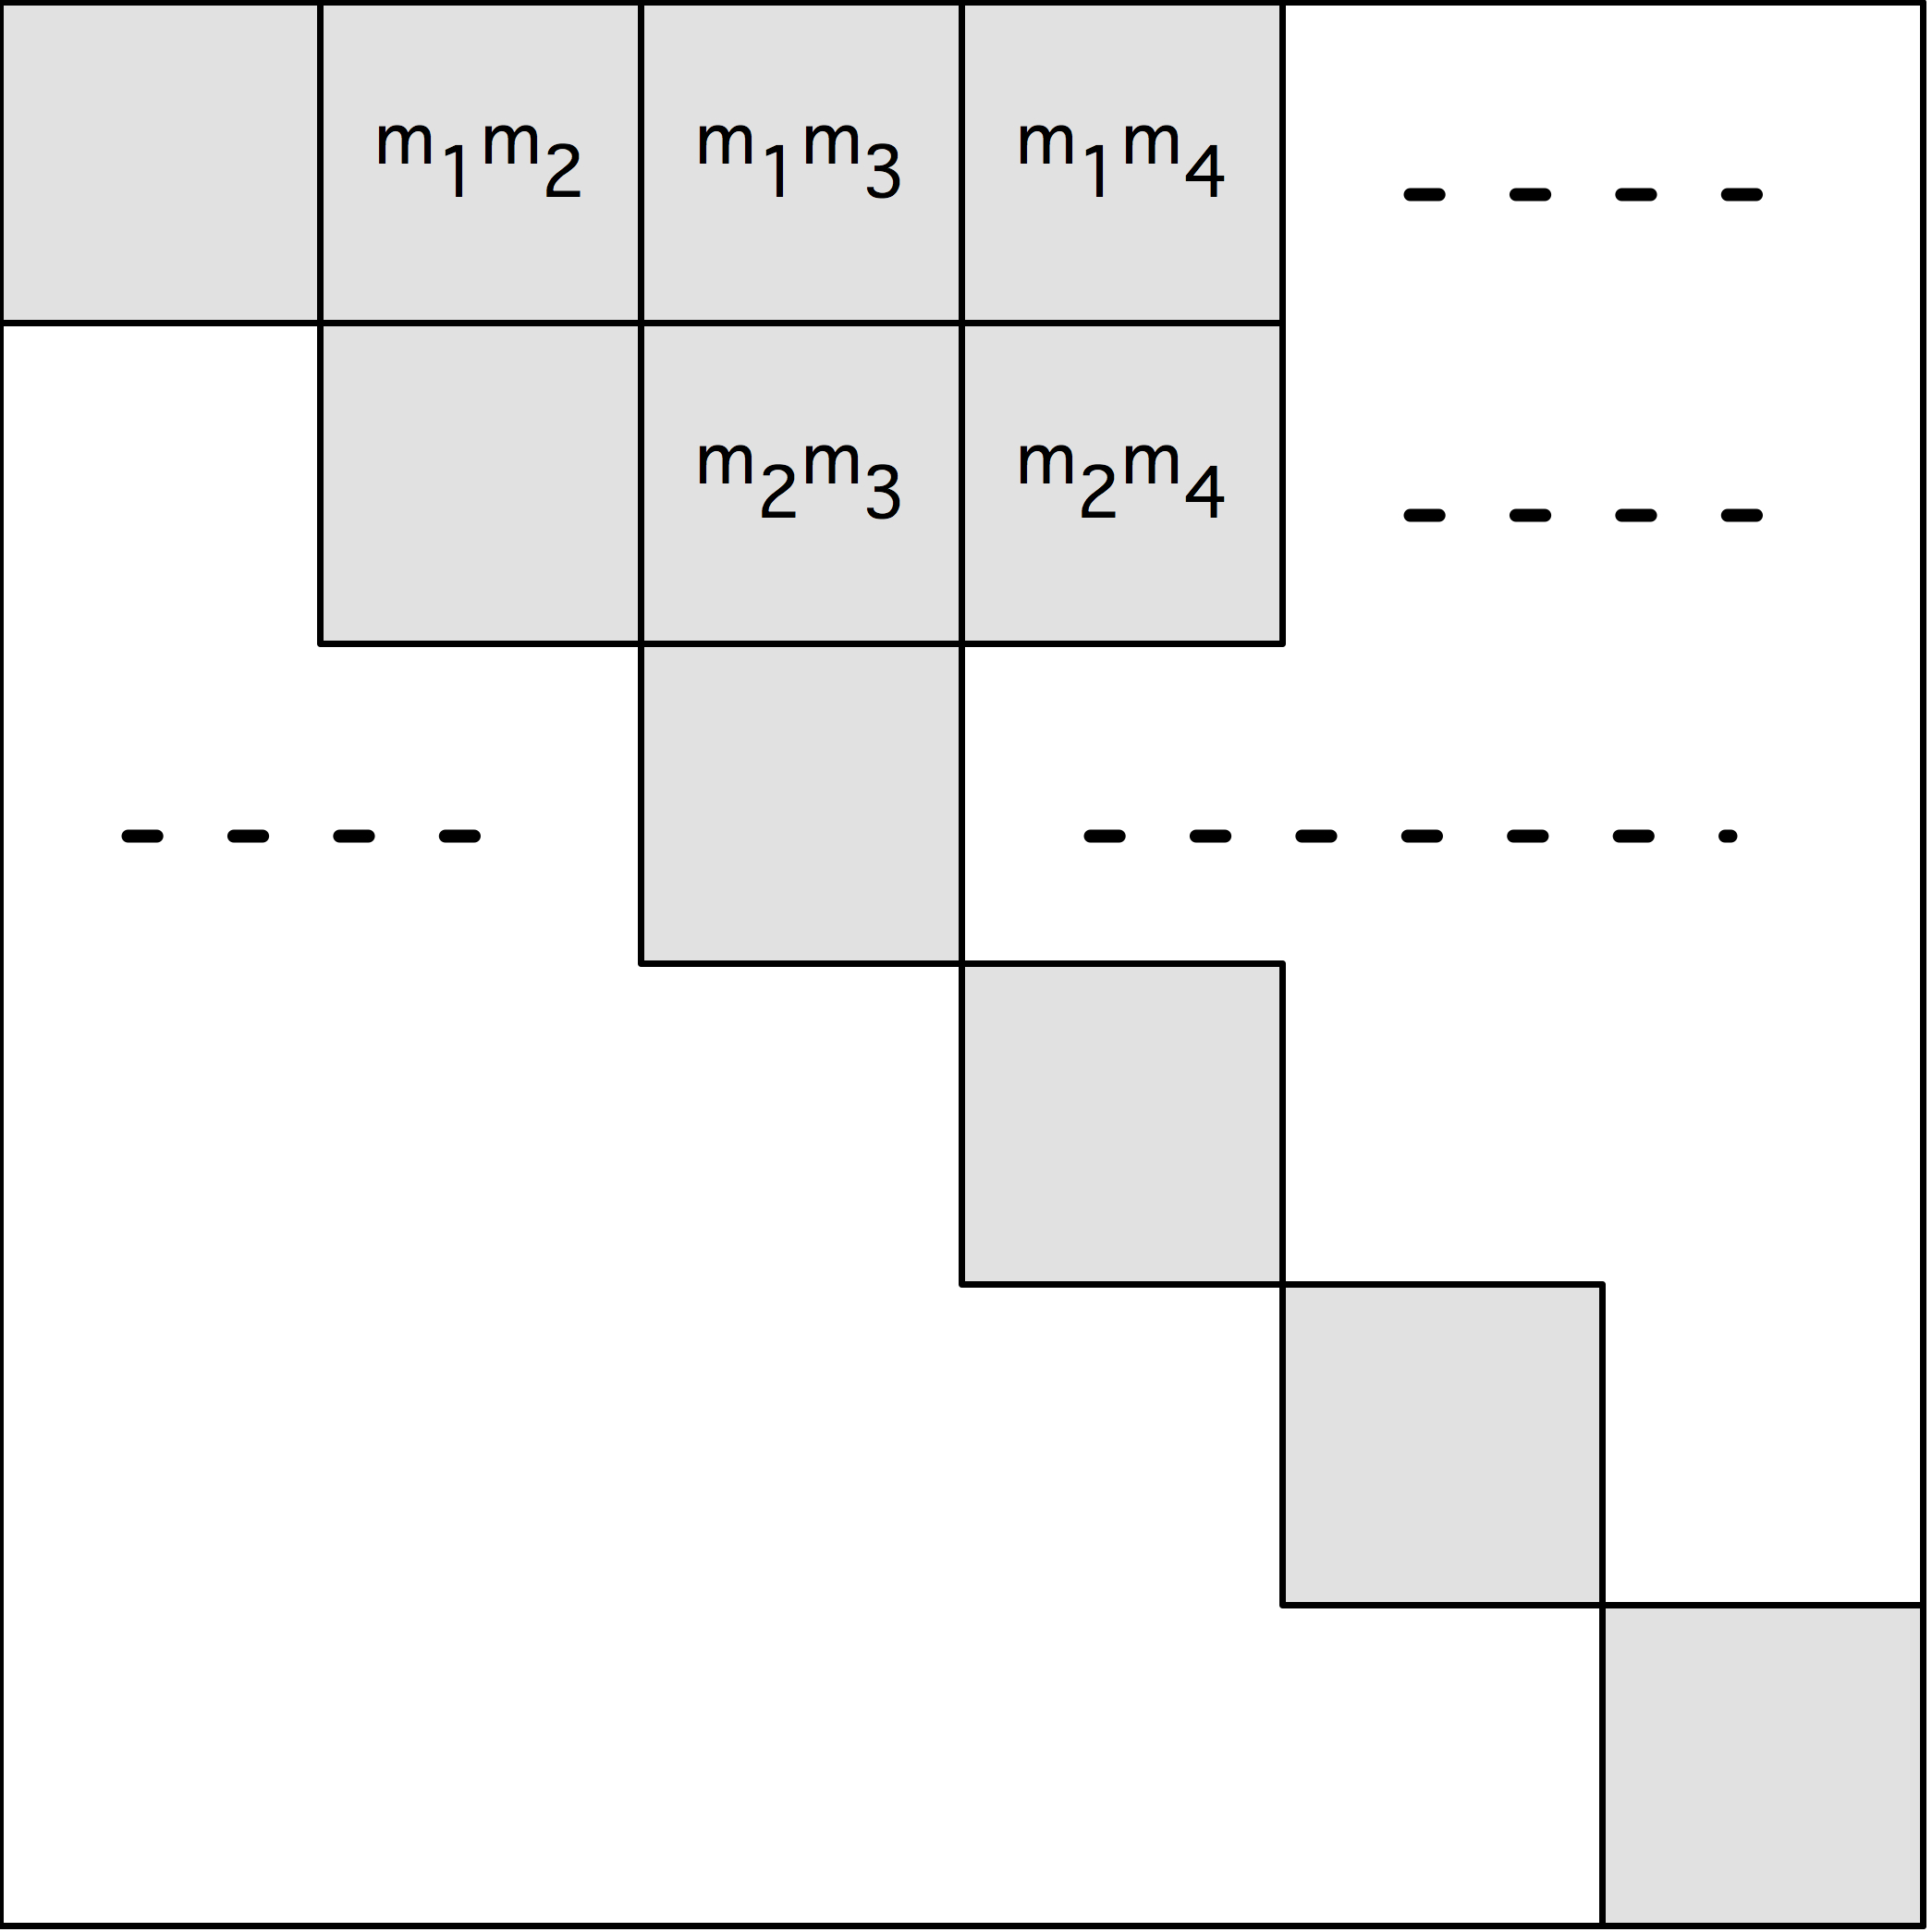
\includegraphics[scale=.1]{all-pairs-pp}
\end{frame}

\begin{frame}
  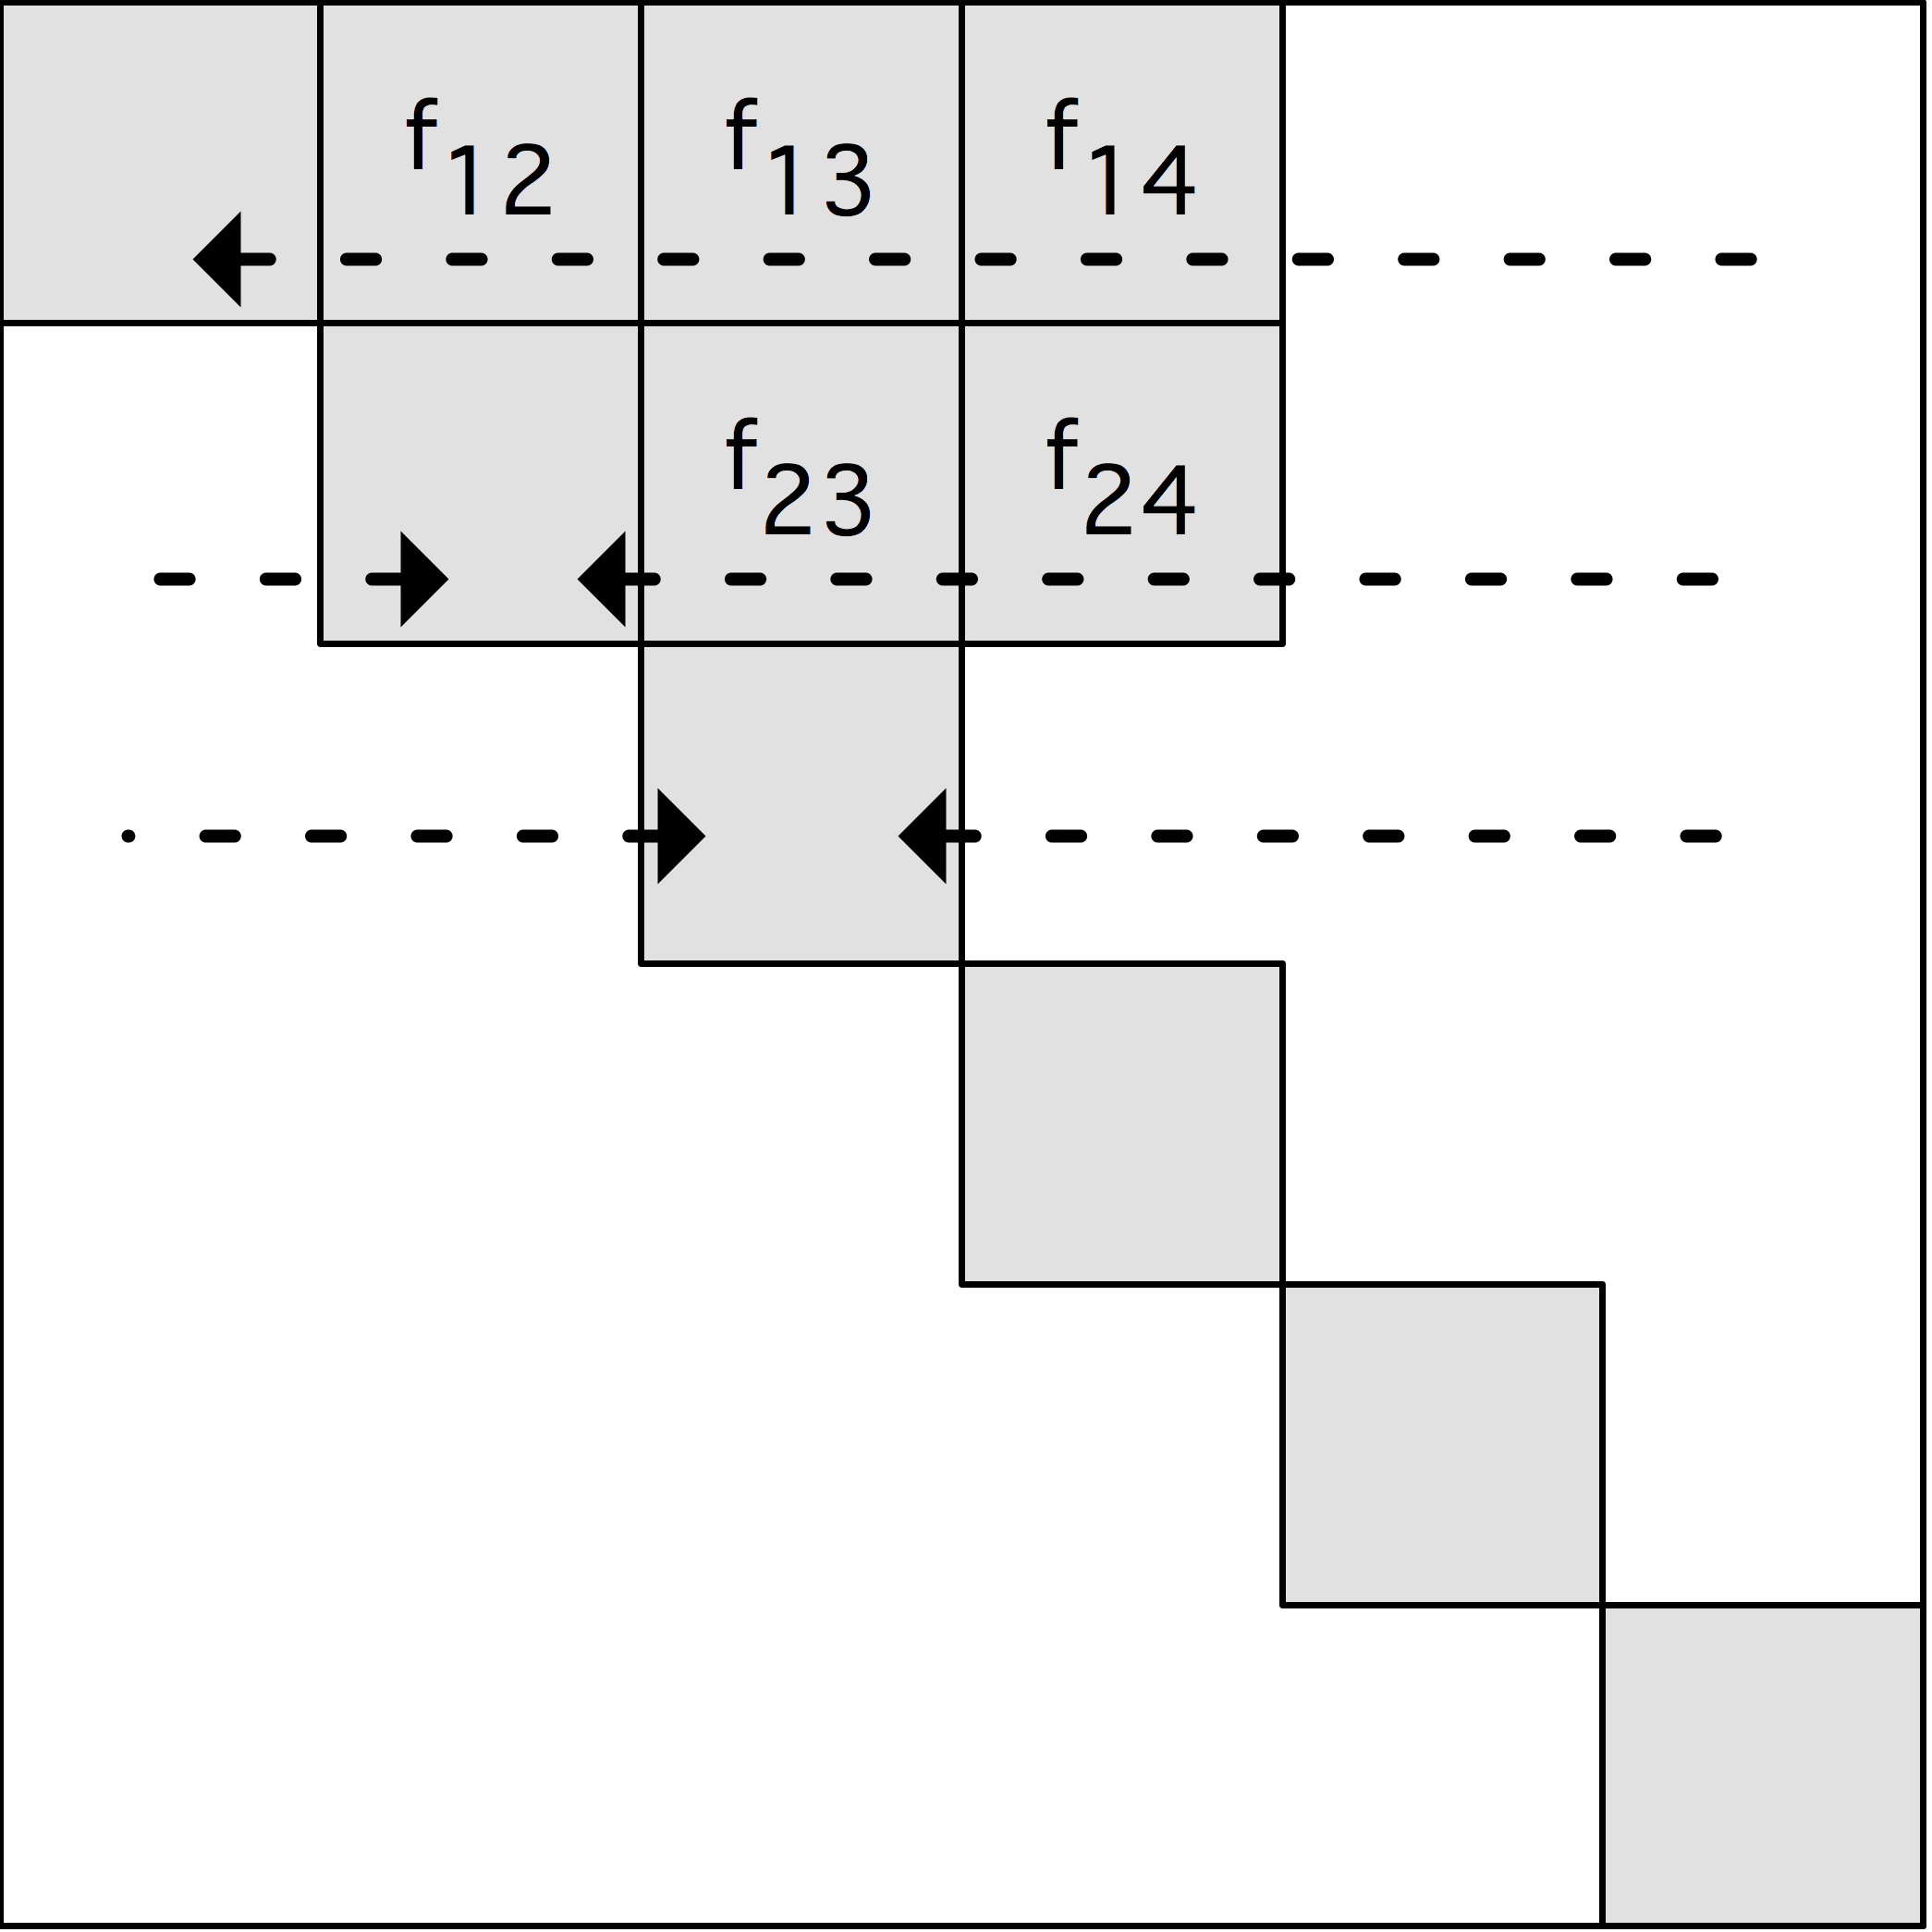
\includegraphics[scale=.1]{all-pairs-f}
\end{frame}

\begin{frame}
  \begin{itemize}
  \item Better algorithm: use $\sqrt P\times\sqrt P$ processor grid,
  \item Divide particles in boxes of $M=N/\sqrt P$
  \item Processor $(i,j)$ computes interaction of boxes $i$ and~$j$:
  \item this requires broadcast (for duplication) and reduction (for
    summing) in processor rows and columns
  \item Bandwidth cost $\beta N/\sqrt P$ which is $M$: scalable.
  \end{itemize}
\end{frame}
